\documentclass[12pt,a4paper,oneside]{report}

% Compile with XeLaTeX and Biber. WMG specifies 12-point text but does not
% mandate a font family. Verdana is currently selected only to resemble the
% supplied Word template and can be changed here without altering the layout.
\usepackage{fontspec}
\setmainfont{Verdana}
\setsansfont{Verdana}
\usepackage[british]{babel}
\usepackage[a4paper,left=25.4mm,right=25.4mm,top=25.4mm,bottom=25.4mm]{geometry}
\usepackage{setspace}
\onehalfspacing
\usepackage{microtype}
\usepackage{csquotes}
\usepackage{graphicx}
\usepackage{tikz}
\usetikzlibrary{arrows.meta,calc,fit,positioning,shapes.geometric}
\usepackage{booktabs}
\usepackage{longtable}
\usepackage{tabularx}
\usepackage{array}
\usepackage{enumitem}
\usepackage{amssymb}
\usepackage{xcolor}
\usepackage{caption}
\usepackage{titlesec}
\usepackage{fancyhdr}
\usepackage[hidelinks]{hyperref}
\usepackage[nameinlink,noabbrev]{cleveref}
\usepackage[
  backend=biber,
  style=authoryear,
  sorting=nyt,
  giveninits=true,
  maxcitenames=2,
  maxbibnames=99,
  uniquename=false,
  dashed=false,
  doi=true,
  url=true,
  isbn=false
]{biblatex}
\addbibresource{references.bib}
% Warwick Harvard in-text citations use a comma between author and year.
\renewcommand*{\nameyeardelim}{\addcomma\space}

\definecolor{wmgblue}{HTML}{2E74B5}
\definecolor{wmgdarkblue}{HTML}{1F4D78}

\titleformat{\chapter}[block]
  {\centering\normalfont\fontsize{16}{19}\selectfont\color{wmgblue}}
  {Chapter \thechapter:}{0.45em}{}
\titleformat{name=\chapter,numberless}[hang]
  {\normalfont\fontsize{16}{19}\selectfont\color{wmgblue}}
  {}{0pt}{}
\titlespacing*{\chapter}{0pt}{0pt}{12pt}
\titleformat{\section}
  {\normalfont\fontsize{13}{16}\selectfont\color{wmgblue}}
  {\thesection}{1em}{}
\titleformat{\subsection}
  {\normalfont\fontsize{12}{15}\selectfont\color{wmgdarkblue}}
  {\thesubsection}{1em}{}
\titleformat{\subsubsection}
  {\normalfont\itshape\color{wmgblue}}
  {\thesubsubsection}{1em}{}

\captionsetup{font={small,it},labelfont=it,justification=centering}
\setlist{itemsep=3pt,topsep=5pt}
\setlength{\parindent}{0pt}
\setlength{\parskip}{8pt}
% Allow modest inter-word flexibility before LaTeX creates an overfull line.
% This is especially useful with 12-point Verdana and Harvard references.
\setlength{\emergencystretch}{3em}

\pagestyle{fancy}
\fancyhf{}
\fancyfoot[R]{\thepage}
\renewcommand{\headrulewidth}{0pt}

\newcommand{\projecttitle}{Design and Evaluation of a Lightweight Complete-Outfit Recommendation System Using Frozen SigLIP Representations, Task-Specific Compatibility Learning and Constrained Candidate Search}
\newcommand{\studentname}{[Student name]}
\newcommand{\studentid}{[Student ID]}
\newcommand{\submissiondate}{[Month Year]}
\newcommand{\checkedbox}{$\boxtimes$}
\newcommand{\emptybox}{$\square$}

\begin{document}

\begin{titlepage}
\thispagestyle{empty}
{\fontsize{16}{19}\selectfont\color{wmgblue}Project Submission Pro-Forma}

\vspace{1.2cm}
Student name: \studentname

Student ID: \studentid

\vspace{0.4cm}
I wish the dissertation to be considered for the course (select one only):

\checkedbox\ MSc in Applied Artificial Intelligence

\vspace{0.4cm}
I confirm that I have included in my dissertation:

\begin{itemize}[label=\emptybox,leftmargin=2em]
  \item An abstract of the work completed
  \item A declaration of my contribution to the work and its suitability for the degree
  \item A table of contents
  \item A list of figures and tables (if applicable)
  \item A glossary of terms (where appropriate)
  \item A clear statement of my project objectives
  \item A full reference list using the Warwick Harvard style
  \item An appendix containing email confirmation of ethical approval or waiver
\end{itemize}

Ethical Approval Waived.

\vfill
Signed: \rule{6cm}{0.4pt}\hfill Date: \rule{3cm}{0.4pt}
\end{titlepage}


\pagenumbering{roman}
\begin{titlepage}
\thispagestyle{plain}
\centering
\IfFileExists{assets/wmg-logo.jpeg}{
  
\includegraphics[width=0.48\textwidth]{assets/wmg-logo.jpeg}
}{
  {\fontsize{28}{34}\selectfont\bfseries WMG\par}
  {\large The University of Warwick\par}
}

\vspace{1.6cm}
{\fontsize{28}{34}\selectfont \projecttitle\par}
\vspace{0.5cm}
by

\vspace{0.4cm}
{\large \studentname, [qualifications obtained]\par}

\vspace{1.5cm}
Dissertation submitted in partial fulfilment for the Degree of Master of Science in Applied Artificial Intelligence

\vfill
\begin{flushright}
WMG\\
University of Warwick
\end{flushright}

\vfill
Submitted \submissiondate
\end{titlepage}

% The title page is preliminary page i. Continue at ii rather than restarting.
\setcounter{page}{2}
\chapter*{Declaration}
\addcontentsline{toc}{chapter}{Declaration}

I have read and understood the rules on cheating, plagiarism and appropriate
referencing as outlined in my handbook and I declare that the work contained
in this assignment is my own, unless otherwise acknowledged.

No substantial part of the work submitted here has also been submitted by me
in other assessments for this or previous degree courses, and I acknowledge
that if this has been done an appropriate reduction in the mark I might
otherwise have received will be made.

\textbf{Project definition for my degree:} [Insert the exact wording from the
Specific Course Regulations for MSc Applied Artificial Intelligence.]

\textbf{Relationship of this project to the degree definition:} [To be written
after the exact course-regulation wording has been verified. This declaration
must remain within one page.]

\clearpage

\chapter*{Abstract}
\addcontentsline{toc}{chapter}{Abstract}

Complete-outfit recommendation requires a system to model relationships among
garments while respecting practical constraints and the item already selected
by a user. This study evaluates whether a small project-specific compatibility
head can support that task without retraining a large visual encoder or tying
the output to a single retailer catalogue. Frozen 768-dimensional SigLIP image
representations were combined with a 379,265-parameter compatibility head and
trained on the published Polyvore Outfits disjoint compatibility split. Here,
\emph{lightweight} refers to the trainable head and its downstream training
cost, not to the size or original pretraining cost of SigLIP. The
model was compared with non-learned, linear, recurrent, type-aware and
attention-based controlled baselines over three random seeds. Evaluation included
classification, corrected FITB ranking, calibration, structural ablation,
imbalance, overfitting, runtime, bias and domain shift.

The selected compatibility model achieved a held-out ROC--AUC of 0.8583 (95\%
bootstrap confidence interval 0.8524--0.8641) and 60.25\% FITB accuracy (95\%
confidence interval 58.73--61.75). The three-seed mean FITB result was 59.94\%.
Removing the pairwise relationship module reduced mean FITB by 10.28 percentage
points, with a paired 95\% interval of 8.96--11.57 points; the smaller gain from
slot embeddings was inconclusive. Training AUC was 0.9699. After
validation-based early stopping, validation and test AUC differed by only
0.00145.

The model was integrated into an abstract, product-independent candidate space
with weather and clothing-range constraints. Exact search exposed substantial
loss from the previous quota path, which recovered the exact top result in
27.78\% of 18 controlled queries. The findings support the feasibility of an
auditable system with lightweight downstream training within the tested
setting. Evaluation was limited by 29.50\% official FITB coverage, sparse
pure-menswear evidence, residual item-identifier overlap across the published
split files, strong catalogue domain shift and the absence of participant
evaluation.

\textbf{Keywords:} fashion recommendation; outfit compatibility; SigLIP;
fill-in-the-blank; constrained search; responsible artificial intelligence

\clearpage

\chapter*{Acknowledgements}
\addcontentsline{toc}{chapter}{Acknowledgements}

[Optional. To be completed by the student.]

\clearpage


\tableofcontents
\clearpage
\listoftables
\clearpage
\listoffigures
\clearpage

% The body margins reproduce the approximately 0.59-inch margins used by the
% supplied WMG template. Change only if WMG publishes a superseding rule.
\newgeometry{left=15mm,right=15mm,top=15mm,bottom=15mm,includeheadfoot}
\pagenumbering{arabic}

\chapter{Introduction}

\section{Background and context}

Digital fashion recommendation covers several related but distinct tasks,
including the retrieval of visually similar products, the identification of
substitutes, individual-item recommendation and the assessment of whether a
set of garments forms a coherent outfit. Visual resemblance alone is
insufficient for the final task. Two shirts may be substitutes because they
serve a similar role, whereas a shirt, trousers and shoes may be complements
because their different roles form a plausible ensemble. Early image-based
recommendation research formalised this distinction between visual similarity,
substitution and complementarity \parencite{mcauley2015styles}. A modern review
similarly characterises fashion recommendation as a domain in which visual,
semantic, contextual and user-related signals interact, while identifying
evaluation, explanation and bias as continuing challenges
\parencite{deldjoo2023review}.

Outfit compatibility research has moved beyond manually specified
colour or category rules towards learned relationships among items. A
bidirectional long short-term memory model represented outfits as ordered
garment sequences and learned their compatibility \parencite{han2017bilstm}.
Type-aware embedding spaces subsequently distinguished similarity from
compatibility across different item relationships
\parencite{vasileva2018typeaware}. OutfitTransformer then used
task-specific tokens and self-attention to model outfit-level relationships
for compatibility prediction and complementary-item retrieval
\parencite{sarkar2023outfittransformer}. These approaches demonstrate that
complete-outfit recommendation is relational: a candidate should be assessed
in the context of the other garments rather than scored as an isolated item.
They also demonstrate that architecture, category representation, negative
construction and evaluation task affect what a reported score means.

Large-scale vision--language pre-training provides a potential representation
layer for smaller downstream studies. SigLIP uses independent sigmoid losses
over image--text pairs instead of requiring softmax normalisation across a
global batch, and was evaluated as a transferable vision--language
representation by \textcite{zhai2023siglip}. A frozen SigLIP image
encoder can supply reusable features while a smaller model learns
the project-specific relationship among garments. Freezing does not make the
representation neutral or guarantee transfer to fashion data; it instead
reduces the number of trainable parameters and makes controlled comparisons
feasible within the resources of an MSc project.

Throughout this dissertation, \emph{lightweight} describes the project-specific
compatibility head and the cost of downstream training on precomputed features.
It does not describe the size or original pretraining cost of the SigLIP
encoder on which those features depend.

\section{Problem definition and motivation}

This dissertation studies a practical complete-outfit task. A user supplies
one garment, and the system recommends abstract garment types and colours for
the remaining supported positions. The prototype, named \emph{Cove}, uses four
logical slots: an inner top, an optional outer layer, a bottom and shoes. The
selected garment remains fixed. Weather conditions, selected style and the
user-selected clothing range constrain the candidate space, while alternatives
allow the user to retain control over the final choice.

The learned problem is complete-outfit compatibility scoring followed by
candidate ranking. This is separated from candidate feasibility. For example,
weather logic may suppress an outer layer in hot conditions, and slot rules
prevent two bottoms from occupying the same outfit. Such constraints should
not be inferred indirectly from a compatibility score. The deployed system
combines a learned relational score with explicit constraints and a
deterministic fallback.

The candidate representation is also deliberately product-independent.
Recommendations are expressed as abstract garment states defined by slot,
broad type, colour, style and clothing range. The states are derived from
secondary Polyvore training data. This design reflects the intended
interaction: a recommendation can
guide the use of an existing wardrobe or a later purchase without claiming
that one retailer contains the only suitable solution. Product-independent
candidate generation also creates a search problem because compatibility is a
non-additive score over complete combinations. The study consequently examines
whether bounded exact search produces materially different results from an
earlier quota-limited retrieval path.

The motivation is both methodological and practical. A large end-to-end model
would be difficult to train, compare and audit with the available time and
computing resources. A rules-only system is transparent but cannot learn the
relationships observed in outfits. The adopted middle position retains a
frozen visual representation, trains a comparatively small compatibility head
and evaluates the learned component separately from the contextual rules and
search procedure.

Figure~\ref{fig:functional-scope} summarises the system boundary from user and
context inputs to the functions that produce and preserve recommendations. It
also distinguishes learned compatibility ranking from recognition, explicit
constraints and wardrobe management. Cove is treated as a
context-aware complete-outfit recommender system. Search is the mechanism used
to explore and rank feasible candidate combinations, rather than a separate
product-search claim.

\begin{figure}[htbp]
  \centering
  \resizebox{\textwidth}{!}{%
  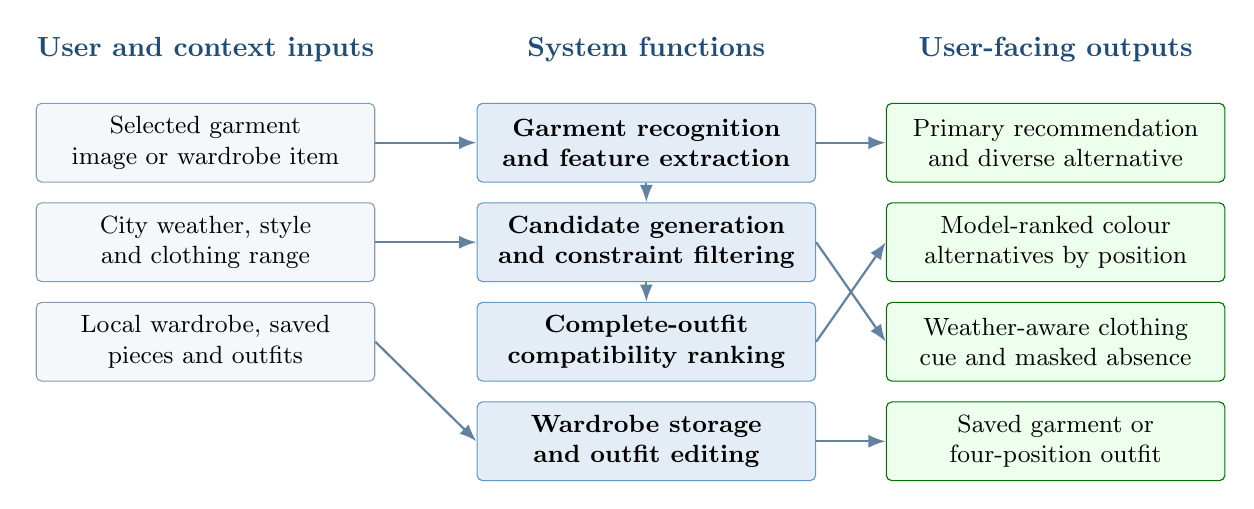
\begin{tikzpicture}[
    font=\small,
    box/.style={draw=wmgdarkblue!55, rounded corners=2pt, minimum width=43mm,
      minimum height=10mm, align=center, fill=wmgblue!5},
    service/.style={box, fill=wmgblue!13, draw=wmgblue!75, font=\small\bfseries},
    output/.style={box, fill=green!7, draw=green!45!black},
    arrow/.style={-{Latex[length=2.2mm]}, thick, draw=wmgdarkblue!70}
  ]
    \node[font=\bfseries\color{wmgdarkblue}] (inputtitle) {User and context inputs};
    \node[box, below=4mm of inputtitle] (garment) {Selected garment\\image or wardrobe item};
    \node[box, below=2.5mm of garment] (context) {City weather, style\\and clothing range};
    \node[box, below=2.5mm of context] (wardrobe) {Local wardrobe, saved\\pieces and outfits};

    \node[font=\bfseries\color{wmgdarkblue}, right=17mm of inputtitle] (servicetitle) {System functions};
    \node[service, below=4mm of servicetitle] (recognition) {Garment recognition\\and feature extraction};
    \node[service, below=2.5mm of recognition] (generation) {Candidate generation\\and constraint filtering};
    \node[service, below=2.5mm of generation] (ranking) {Complete-outfit\\compatibility ranking};
    \node[service, below=2.5mm of ranking] (management) {Wardrobe storage\\and outfit editing};

    \node[font=\bfseries\color{wmgdarkblue}, right=17mm of servicetitle] (outputtitle) {User-facing outputs};
    \node[output, below=4mm of outputtitle] (primary) {Primary recommendation\\and diverse alternative};
    \node[output, below=2.5mm of primary] (replacement) {Model-ranked colour\\alternatives by position};
    \node[output, below=2.5mm of replacement] (weather) {Weather-aware clothing\\cue and masked absence};
    \node[output, below=2.5mm of weather] (saved) {Saved garment or\\four-position outfit};

    \draw[arrow] (garment.east) -- (recognition.west);
    \draw[arrow] (context.east) -- (generation.west);
    \draw[arrow] (wardrobe.east) -- (management.west);
    \draw[arrow] (recognition.east) -- (primary.west);
    \draw[arrow] (generation.east) -- (weather.west);
    \draw[arrow] (ranking.east) -- (replacement.west);
    \draw[arrow] (management.east) -- (saved.west);
    \draw[arrow] (recognition) -- (generation);
    \draw[arrow] (generation) -- (ranking);
  \end{tikzpicture}}
  \caption{Functional scope of the Cove complete-outfit recommendation system}
  \label{fig:functional-scope}
\end{figure}


\section{Research gap}

The literature establishes that recurrent, type-aware and attention-based
models can learn fashion compatibility
\parencite{han2017bilstm,vasileva2018typeaware,sarkar2023outfittransformer}.
It does not follow that the most
complex published architecture is automatically the most appropriate model
for a smaller, processed dataset, a frozen visual representation and a
resource-constrained application. Reported results are coupled to dataset
splits, negative construction, candidate availability and evaluation protocol
\parencite{herlocker2004evaluation,vasileva2018typeaware}.
The broader fashion-recommender literature also cautions that offline accuracy
alone does not resolve questions of explanation, bias or operational use
\parencite{deldjoo2023review}.

The gap addressed here is bounded and empirical rather than a claim
that outfit recommendation itself is novel. First, it is uncertain whether a
small relational head on frozen vision--language features can outperform
non-learned and controlled learned alternatives under one consistent
pipeline. Second, aggregate compatibility classification does not establish
candidate-completion quality, calibration or generalisation; corrected FITB,
ablation, repeated seeds and overfitting evidence are also required. Third, a
model score does not by itself specify how a practical system should explore a
large abstract candidate space under weather and clothing-range constraints.
The project addresses these questions jointly while keeping model evaluation
distinct from claims about human taste or satisfaction.

\section{Research question}

The primary research question is:

\begin{quote}
To what extent can a small project-specific outfit-compatibility head built on frozen
vision--language embeddings, combined with exact constrained search over
abstract garment states, provide accurate, computationally practical and
auditable complete-outfit recommendations using secondary fashion data?
\end{quote}

Three sub-questions operationalise the model and system components:

\begin{description}[style=nextline,leftmargin=1.2cm,labelindent=0cm]
  \item[\textbf{RQ1.}] How does the proposed compatibility model compare with
        non-learned and controlled learned baselines under consistent data and
        evaluation protocols?
  \item[\textbf{RQ2.}] Which architectural and training choices are supported
        by compatibility classification, corrected FITB, calibration,
        ablation and generalisation evidence?
  \item[\textbf{RQ3.}] What completeness, latency and control trade-offs arise
        when quota-limited retrieval is replaced by exact constrained search
        over product-independent abstract garment states?
\end{description}

The wording \emph{to what extent} requires negative as well as positive
evidence. A high AUC is treated as evidence of discrimination, not as the
percentage of recommendations that users will like. Model ranking, uncertainty,
runtime, data coverage, bias and domain shift all contribute to the
answer.

\section{Research objectives}

The research question is addressed through the following objectives:

\begin{enumerate}[label=\textbf{O\arabic*.}]
  \item Critically synthesise research on fashion compatibility,
        vision--language representation, recommendation evaluation and
        responsible design, and define a reproducible secondary-data method
        consistent with the approved ethical scope.
  \item Develop and evaluate a lightweight project-specific complete-outfit
        compatibility head
        using frozen SigLIP embeddings, including controlled baselines and
        evidence from classification, FITB, calibration, ablation,
        generalisation, imbalance and uncertainty analyses.
  \item Design and implement a product-independent recommendation prototype
        that combines exact candidate search, explicit contextual constraints,
        local wardrobe management, an interaction design intended to support
        clear and accessible use, and a
        deterministic fallback, then verify its functionality, coverage and
        runtime.
  \item Critically evaluate the confidence, limitations, practical value and
        future deployment opportunities supported by the combined model and
        system evidence.
\end{enumerate}

\section{Scope and boundaries}

The investigation is confined to secondary datasets; no human participants
were recruited for interviews, questionnaires or experiments. The project
received confirmation dated 12 May 2026 that ethical approval was waived. The
required research-integrity, information-security and WMG student-ethics
training evidence, together with the waiver confirmation, is reproduced in
Appendices A and B. The separately published Zara dataset retained locally is
used for recognition and feature-domain diagnostics, not as the sole
recommendation source.

The study does not claim to learn an objective or universal definition of
fashion compatibility. Demographic attributes are not collected, so
demographic fairness and user satisfaction cannot be measured
\parencite{mehrabi2021bias,selbst2019fairness}. The interface
asks the user to choose a menswear or womenswear candidate range; it does not
infer gender from a person or garment image \parencite{keyes2018misgendering}.
Sparse pure-menswear training data
preclude a claim that both ranges have equal model reliability. Long-term
personalisation from clicks is also outside scope because defensible online
learning would require exposure logging, feedback-loop controls and a separate
evaluation design \parencite{chaney2018confounding}. Local wardrobe data do not
retrain the compatibility model.

The evaluated representation is limited to an inner top, optional outer layer,
bottom and shoes. Dresses, jumpsuits and other one-piece garments would require
an explicit multi-slot occupancy representation and separate training and
evaluation. Accessories and culturally specific garment structures are not
modelled comprehensively. Official FITB reporting is restricted to questions
representable by these four slots and available frozen embeddings; coverage is
reported so that the filtered result is not presented as a full official
benchmark score.

The work evaluates offline compatibility and system behaviour, not commercial
conversion or human preference. Earlier engineering models use different
candidate or data protocols and are not treated as causal evidence that one
development stage improves another. Controlled claims are based on
same-split baselines, architecture comparisons, structural ablations and the
exact-versus-quota search experiment.

\section{Contributions}

Within these boundaries, the dissertation makes four contributions. First, it
provides a reproducible compatibility pipeline with lightweight downstream
training that separates a
frozen visual representation, a learned relational head and explicit
contextual constraints. Second, it provides a controlled evaluation comprising
non-learned and learned baselines, three seeds, corrected set-identifier-based
FITB labels, structural ablation, calibration and an explicit overfitting
audit. Third, it develops an abstract candidate representation and evaluates
bounded exact search against a quota-limited retrieval path using the same
deployed objective. Fourth, it demonstrates a local-first prototype in which
the user retains the selected garment, chooses the clothing range, receives
weather-aware alternatives and can fall back to deterministic rules if model
artefacts are unavailable.

The contributions are methodological, empirical and artefactual. The comparison
models are controlled adaptations rather than exact reproductions of the
published architectures.

\section{Dissertation structure}

Chapter 2 critically reviews recommender-system foundations, fashion
compatibility, vision--language representations, candidate search, evaluation
and responsible-system concerns. Chapter 3 specifies the secondary-data
pipeline, model, baselines, experimental protocol, metrics, candidate-search system
and ethical safeguards. Chapter 4 reports the model and system results without
extended interpretation. Chapter 5 analyses model behaviour, architectural
evidence, overfitting and search trade-offs. Chapter 6 relates the findings to
previous research, answers the research questions and evaluates contribution,
validity, practical implications and limitations. Chapter 7 concludes by
assessing the objectives and identifying proportionate future work.

\section{Summary}

This chapter has framed complete-outfit recommendation as relational
compatibility scoring followed by constrained candidate search. It has defined
a bounded empirical gap, one primary research question, three sub-questions
and four objectives. The scope excludes participant claims, online
personalisation and unsupported garment structures, while retaining model,
search, runtime, bias and reproducibility evidence. Chapter 2 now evaluates
the literature from which the representation, compatibility and assessment
choices are derived.

\chapter{Literature Review}

\section{Introduction}

This chapter critically reviews the research underpinning the project's
representation, compatibility-modelling, retrieval and evaluation choices.
Fashion recommendation includes visual similar-item retrieval, substitute
recommendation, personalised ranking, outfit compatibility prediction and
complementary-item retrieval \parencite{deldjoo2023review,sarkar2023outfittransformer}.
Because these tasks differ in their inputs, supervision and definitions of
success, evidence obtained for one cannot automatically support another.

The review first positions complete-outfit recommendation within recommender
systems, then examines the development of fashion-compatibility models and the
role of frozen vision--language representations. It subsequently considers
learning objectives, evaluation, candidate search and responsible design. The
literature is used to derive controlled alternatives, not to assume that the
newest or most complex architecture is necessarily appropriate.

\section{Positioning complete-outfit recommendation}

Traditional recommender systems often learn from interactions such as ratings,
clicks or purchases and ask which item should be presented to a particular
user. Evaluation must be connected to the user task, available observations and
intended use; otherwise, nominally similar experiments may not be comparable
\parencite{herlocker2004evaluation}. Fashion recommenders extend this setting
with visual, textual, contextual and social information
\parencite{deldjoo2023review}.

Cove has no longitudinal user--item history and therefore does not claim to
learn stable individual preferences or compare collaborative-filtering
algorithms. Its learned task is content-based outfit compatibility: estimating
whether relationships within a set of garments resemble those observed in the
training outfits. At runtime, that score ranks completions around a
user-selected garment. Dataset compatibility and personal preference must
remain distinct, because following a dataset regularity does not establish what
one person will prefer.

Complete-outfit recommendation is consequently considered at three connected
levels. Representation converts garment images into features; relational
scoring evaluates garments jointly; decision and interaction filter infeasible
candidates, search combinations and expose alternatives. Secondary outfit data
can evaluate the first two levels. The third can be tested for deterministic
behaviour, completeness and runtime, but not for satisfaction without human
evidence. This separation prevents the compatibility classifier from being
treated as the entire recommender system.

\section{Development of fashion-compatibility models}

Early image-based recommendation distinguished visual similarity from
complementarity. Items serving the same role may be substitutes, whereas items
from different roles may be complementary despite being visually dissimilar
\parencite{mcauley2015styles}. Pairwise metric learning operationalises this
distinction by learning spaces in which compatible pairs are close. Such models
support efficient nearest-neighbour retrieval, but a complete outfit contains
several interacting pairs. Summing local scores assumes that pairwise
compatibility is sufficient to represent the set.

\textcite{han2017bilstm} represented outfits as ordered garment sequences and
used a bidirectional long short-term memory network. This aggregates information
from garments on both sides of an item, although outfits have no natural
linguistic order and must be ordered through garment categories. The method
therefore provides a useful structured baseline while retaining possible
sensitivity to that imposed sequence.

\textcite{vasileva2018typeaware} argued that compatibility depends on item type
and proposed type-aware embedding spaces. A top--shoe relationship need not use
the same transformation as a top--top relationship, making category or slot
identity part of the learned relation rather than descriptive metadata. This
supports testing slot-pair-specific projections and explicit slot
representations.

Context-aware graph modelling provides another response to isolated pair
relations. \textcite{cucurull2019context} generated product embeddings
conditioned on known compatible context and reported stronger compatibility
prediction when more context was available. The finding supports the view that
compatibility is conditional rather than intrinsic to one item. Graph
construction requires available nodes and edges, which may not exist for a
newly uploaded garment.

Attention allows each garment representation to interact with every other
garment without requiring a fixed sequence. OutfitTransformer uses task-specific
tokens and self-attention for outfit compatibility and complementary-item
retrieval \parencite{sarkar2023outfittransformer}. Treating an outfit as an
unordered set is appropriate because rearranging the same garments should not
change compatibility. Attention offers flexible higher-order interaction but
also adds capacity. Results obtained under OutfitTransformer's original
protocol do not establish that equal capacity is required with frozen inputs
and a smaller processed dataset.

These studies support several modelling assumptions rather than one universal
architecture. Pairwise models prioritise local relations and efficiency;
recurrent models learn structured aggregation; type-aware models encode
category-dependent relations; and attention learns set-level interactions
\parencite{han2017bilstm,vasileva2018typeaware,sarkar2023outfittransformer}.
Their differences motivate controlled comparisons using the same features,
splits and training conditions.

\section{Polyvore data and label construction}

Polyvore datasets convert outfits assembled by platform users into observable
item sets and are consequently practical secondary data for compatibility
research \parencite{han2017bilstm,vasileva2018typeaware}. A positive example
records an outfit retained in the dataset; it is not evidence of an objective
or universally shared aesthetic judgement.

Negative outfits are commonly constructed by replacing an item in a positive
outfit. Same-type replacement is harder than arbitrary-category replacement
because the negative remains structurally plausible
\parencite{vasileva2018typeaware}. Since replacements are generated rather than
independently judged incompatible, they may include false negatives. This risk
follows from the published construction procedure; it does not establish that
a known proportion of labels is incorrect.

Splitting the data changes the generalisation question. If a product appears in
both training and testing outfits, a model may benefit from recognising an
observed item. Vasileva et al. describe their revised Polyvore partition as a
disjoint split intended to reduce this problem
\parencite{vasileva2018typeaware}. The present project retains that published
name, while independently auditing the locally acquired metadata rather than
assuming complete item-level separation. Such a split also leaves shared
photographic conventions, category distributions, platform culture and
labelling assumptions unchanged.

In the common fill-in-the-blank (FITB) task, one garment is removed and the
model selects the correct completion from four candidates
\parencite{han2017bilstm,vasileva2018typeaware}. FITB evaluates relative ranking
within a small set and is closer to recommendation than binary classification,
but remains smaller than full-catalogue retrieval. OutfitTransformer evaluates
compatibility prediction and large-scale retrieval separately, reinforcing
that FITB does not establish scalable retrieval quality
\parencite{sarkar2023outfittransformer}.

Polyvore is therefore suitable for controlled training and offline evaluation.
It cannot represent all clothing practices. Filtering official questions to
four supported slots introduces an additional coverage boundary. The retained
fraction must accompany the subset result so that it is not presented as the
complete official benchmark.

\section{Frozen vision--language representations}

Earlier compatibility systems commonly used convolutional encoders pretrained
on ImageNet and adapted to fashion data \parencite{vasileva2018typeaware}.
Vision--language models instead learn from large collections of image--text
pairs. CLIP demonstrated transferable visual representations and zero-shot
recognition across numerous downstream datasets \parencite{radford2021clip}.

SigLIP belongs to this family but replaces a global softmax contrastive
objective with independent sigmoid losses over image--text pairs
\parencite{zhai2023siglip}. It was not pretrained for outfit compatibility; its
image encoder instead supplies a general visual representation from which a
smaller downstream model can attempt to learn garment relationships.

Freezing the encoder converts each image into a fixed vector and restricts
training to the compatibility head. For this project, that reduces trainable
parameters, repeated image-processing cost and representation variation across
baselines. It also permits comparisons with identical inputs. These are
computational and experimental advantages within the project, not evidence
that frozen features are universally preferable.

The downstream head cannot recover information absent from the frozen vector.
Transfer is not guaranteed by source-model scale alone:
\textcite{kornblith2019transfer} found that transfer depends on both
representation and target task, with limited benefit on some fine-grained
datasets. Web-scale pretraining can also transmit biases in the source data
\parencite{radford2021clip,mehrabi2021bias}. Frozen SigLIP is thus a
resource-conscious hypothesis to test rather than an assumed fashion-specific
solution.

\section{Learning objectives and controlled baselines}

Compatibility classification and recommendation ranking are related but
distinct. Binary cross-entropy trains separation of labelled positive and
negative outfits. Its score can order candidates, but the loss does not
directly optimise order among competing completions. Pairwise ranking instead
encourages a preferred observation to score above an alternative; Bayesian
Personalised Ranking is one established formulation for implicit observations
\parencite{rendle2009bpr}.

Neither objective is automatically preferable here. Binary labels are directly
available in the compatibility rows, whereas ranking requires defensible
positive--negative pairs. If a synthetic negative is noisy, a ranking objective
may optimise an unreliable comparison. The choice must be evaluated rather
than inferred from the fact that runtime recommendation uses ranking.

The controlled baselines form a hierarchy. Chance provides a lower bound for
four-choice FITB. Non-learned cosine similarity tests whether frozen features
already contain useful structure. A linear model over pooled features tests
whether learned weighting is sufficient without nonlinear interaction. These
controls prevent the downstream architecture from receiving credit for
information already present in SigLIP.

A recurrent baseline represents the sequence assumption of
\textcite{han2017bilstm}; a type-aware model represents relation-specific
transformations from \textcite{vasileva2018typeaware}; and attention represents
set-level interaction following \textcite{sarkar2023outfittransformer}. These
are controlled approximations, not exact reproductions, which would require the
original encoders, preprocessing, objectives and hyperparameters.

Structural ablation addresses component contribution. Removing the pairwise
module tests whether explicit item--item interaction adds evidence beyond
pooled outfit information. Removing slot embeddings tests whether slot identity
adds evidence beyond visual vectors. If removal does not produce a consistent
decline across repeated runs, the component's benefit remains uncertain.

\section{Evaluation beyond a single score}

Evaluation should match the task claimed \parencite{herlocker2004evaluation}.
Compatibility classification, candidate completion, confidence interpretation
and application behaviour therefore require separate evidence.

ROC--AUC measures discrimination across thresholds and can be interpreted as
the probability that a randomly selected positive receives a higher score than
a randomly selected negative \parencite{fawcett2006roc}. It does not measure
whether the correct completion ranks first in a candidate set, nor whether a
score is a calibrated probability.

FITB evaluates completion more directly. In a balanced four-choice question,
chance accuracy is 25\%, but performance still depends on candidate and label
construction. Correct answers must be matched through the documented dataset
relationship rather than assumed to occupy a fixed array position. Retaining
question-level outputs makes label correction and paired comparison auditable.

Calibration is separate from discrimination. Neural networks may rank examples
correctly while remaining overconfident; temperature scaling was effective in
several classification settings examined by \textcite{guo2017calibration}.
Because a positive scalar temperature does not alter logit order, it can improve
confidence interpretation without improving FITB ranking.

Stochastic training variation must also be reported. Parameter initialisation,
data order and other benchmark stages can alter an otherwise unchanged
experiment \parencite{bouthillier2021variance}. Cove uses three seeded runs for
its principal architecture comparisons. This is a resource-constrained
repeated-run design, not a complete characterisation of training variance.

Structural ablations are evaluated on the same FITB questions and matched
seeds. Pairing preserves the full--ablation relationship on each evaluation
unit instead of treating their predictions as independent
\parencite{dietterich1998tests}. The project's bootstrap averages the three
seeded outcomes within each question and then resamples questions, following
the bootstrap principle of estimating sampling uncertainty by resampling
\parencite{efron1994bootstrap}. Its interval is conditional on those runs and
does not represent every possible training seed.

Overfitting is examined through training, validation and held-out test
behaviour. Validation-based early stopping is intended to stop iterative
training when further training improvement is no longer accompanied by better
validation performance \parencite{prechelt1998early}. A small
validation--test difference supports only the consistency of the selected
checkpoint on the current test split, not general reliability. Stronger
training than validation and test performance is consistent with training-set
overfitting, although data composition can also contribute.

No offline metric establishes user benefit. Without participant evidence,
claims remain limited to discrimination, controlled completion ranking,
calibration, runtime, coverage and deterministic system behaviour.

\section{Candidate search and explicit constraints}

A model scores only candidates that reach it. If a strong candidate is removed
by a frequency quota or similarity shortlist, later ranking cannot recover it.
Candidate generation is therefore part of recommendation behaviour rather than
neutral preprocessing.

Large-scale complementary-item systems commonly use embedding retrieval.
OutfitTransformer creates a target representation and applies nearest-neighbour
retrieval \parencite{sarkar2023outfittransformer}. Vector indexes and
approximate search make this efficient at very large scale, trading retrieval
completeness for speed or memory \parencite{johnson2021similarity}.

Cove instead assigns a non-additive score to a complete combination. An item
that is not individually closest to the uploaded garment can still participate
in the highest-scoring complete outfit, so independent slot shortlists may not
preserve the final optimum. This follows from the deployed scoring function
rather than from a claim made by the retrieval literature.

For a bounded four-slot space, batched exhaustive scoring can remain feasible.
Here, \emph{exact} means that every combination surviving the declared filters
is evaluated under one deployed objective. A safety limit is required so an
oversized search fails explicitly rather than presenting a partial prefix as
complete.

Weather suitability, slot occupancy and the user-selected clothing range are
feasibility requirements, not aesthetic preferences inferred from Polyvore.
The model ranks feasible outfits, while deterministic rules define what is
allowed. This keeps model behaviour, search completeness and functional
constraints separately auditable.

\section{Bias, personalisation and responsible design}

Bias can enter through data selection, labels, pretrained representations,
candidate construction and interaction design, and cannot be reduced to
overall accuracy \parencite{mehrabi2021bias}. Clothing practice is also
cultural, temporal and subjective \parencite{deldjoo2023review}.

Polyvore reflects a historical platform population and may over-represent some
categories, presentation styles and commercial photography. Synthetic
same-type negatives add another assumption, while SigLIP carries uncertainty
from web-scale pretraining. These sources justify an audit and explicit
limitations, but do not permit demographic fairness to be measured without
demographic attributes.

Automatic gender inference would add an uncertain identity classification, a
practice criticised in human--computer interaction research
\parencite{keyes2018misgendering}. Cove asks the user to choose a menswear or
womenswear candidate range instead. Those terms remain simplified catalogue
filters and are not definitions of the user.

Local execution reduces external transmission of wardrobe data but does not
resolve feedback bias. Exposure influences which clicks become observable, and
simulation evidence shows that algorithmically confounded feedback can
increase behavioural homogeneity without increasing utility
\parencite{chaney2018confounding}. Defensible long-term self-learning would
need exposure logging, exploration, feedback-loop controls and separate
evaluation, so it lies outside the frozen study.

Fairness cannot be detached from social context or treated solely as a property
of an isolated component \parencite{selbst2019fairness}. A proportionate
response documents limitations, avoids identity inference, retains the
selected garment, exposes alternatives and permits rejection or replacement.

\section{Synthesis and research framework}

The literature supports four conclusions. First, compatibility is relational:
visual similarity is insufficient and category identity can form part of the
relation, although maximum model complexity is not always justified
\parencite{mcauley2015styles,vasileva2018typeaware,sarkar2023outfittransformer}.
This supports evaluating a lightweight relational head against progressively
stronger alternatives.

Second, frozen vision--language features offer a feasible representation
strategy rather than a fashion-specific solution. They reduce training burden
while retaining transfer, domain and inherited-bias risks
\parencite{radford2021clip,zhai2023siglip,kornblith2019transfer}. The downstream
head must consequently be compared with non-learned and learned controls.

Third, ROC--AUC, FITB, calibration, repeated runs, ablation, coverage and domain
diagnostics answer different questions
\parencite{fawcett2006roc,guo2017calibration,bouthillier2021variance}.

Fourth, candidate generation and explicit constraints affect deployed
behaviour as well as scoring. Approximate retrieval is appropriate at very
large scale, but a bounded non-additive four-slot objective creates a testable
case for exact constrained search
\parencite{sarkar2023outfittransformer,johnson2021similarity}.

The remaining empirical questions are whether a small relational head on
frozen SigLIP features can balance discrimination, completion ranking, runtime
and auditability under one secondary-data protocol, and how much deployed-model
quality is lost through quota candidate generation. Chapter 3 translates those
questions into controlled experiments.

\section{Summary}

Cove has been positioned as a content-based compatibility and constrained-search
system rather than a conventional personalised collaborative recommender. The
literature shows a progression from pairwise visual relations to sequence,
type-aware, contextual and attention-based modelling. It supports frozen
vision--language features as a resource-conscious experimental layer while
requiring explicit treatment of transfer, labels, evaluation and bias.

Chapter 3 applies this framework through the methodology used for model and
system evaluation.

\chapter{Methodology}

\section{Research approach}

This project used a quantitative secondary-data approach combined with
software-system evaluation. The investigation examined whether a small
project-specific head could learn outfit compatibility from published fashion data and whether
its scores could support a practical recommendation application. The research
therefore covered both model performance and the behaviour of the complete
recommendation process.

The project did not conduct interviews, questionnaires or other participant
research. The available evidence is limited to offline model evaluation,
controlled comparisons and functional system testing.

The complete technical route is shown in Figure~\ref{fig:technical-route}.
It separates secondary-data preparation and frozen feature extraction from
compatibility learning, controlled evaluation and application deployment.

\begin{figure}[htbp]
  \centering
  \resizebox{\textwidth}{!}{%
  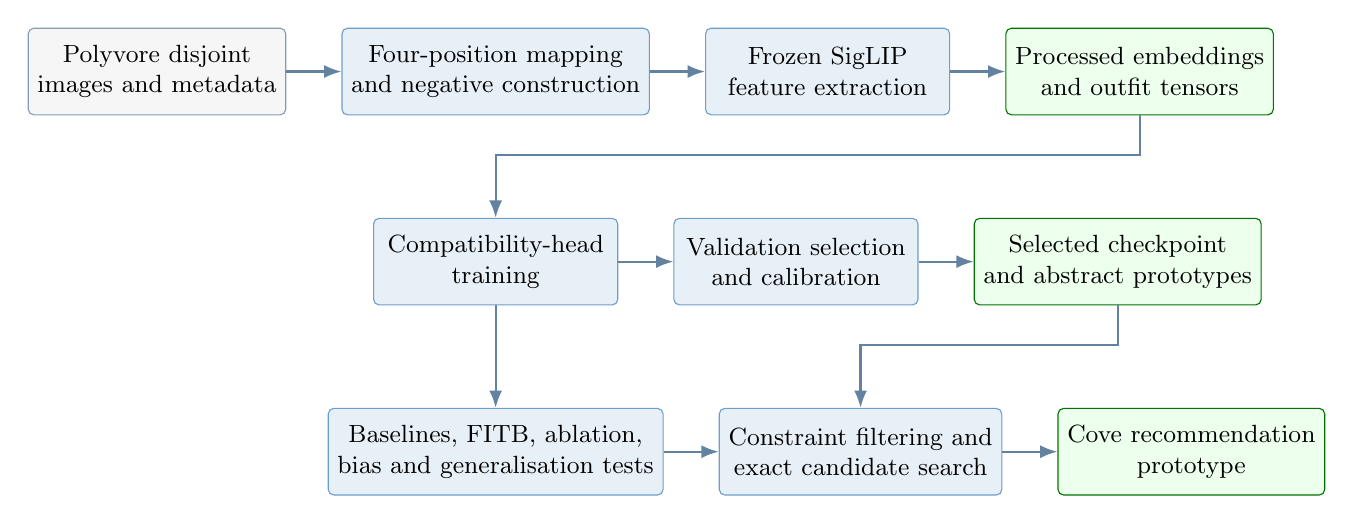
\begin{tikzpicture}[
    font=\small,
    data/.style={draw=wmgdarkblue!55, rounded corners=2pt, align=center,
      minimum width=31mm, minimum height=11mm, fill=gray!7},
    process/.style={data, fill=wmgblue!11, draw=wmgblue!70},
    artefact/.style={data, fill=green!7, draw=green!45!black},
    arrow/.style={-{Latex[length=2.2mm]}, thick, draw=wmgdarkblue!70}
  ]
    \node[data] (polyvore) {Polyvore disjoint\\images and metadata};
    \node[process, right=7mm of polyvore] (mapping) {Four-position mapping\\and negative construction};
    \node[process, right=7mm of mapping] (siglip) {Frozen SigLIP\\feature extraction};
    \node[artefact, right=7mm of siglip] (tensors) {Processed embeddings\\and outfit tensors};

    \node[process, below=13mm of mapping] (training) {Compatibility-head\\training};
    \node[process, right=7mm of training] (selection) {Validation selection\\and calibration};
    \node[artefact, right=7mm of selection] (checkpoint) {Selected checkpoint\\and abstract prototypes};

    \node[process, below=13mm of training] (evaluation) {Baselines, FITB, ablation,\\bias and generalisation tests};
    \node[process, right=7mm of evaluation] (runtime) {Constraint filtering and\\exact candidate search};
    \node[artefact, right=7mm of runtime] (prototype) {Cove recommendation\\prototype};

    \draw[arrow] (polyvore) -- (mapping);
    \draw[arrow] (mapping) -- (siglip);
    \draw[arrow] (siglip) -- (tensors);
    \draw[arrow] (tensors.south) -- ++(0,-5mm) -| (training.north);
    \draw[arrow] (training) -- (selection);
    \draw[arrow] (selection) -- (checkpoint);
    \draw[arrow] (checkpoint.south) -- ++(0,-5mm) -| (runtime.north);
    \draw[arrow] (training) -- (evaluation);
    \draw[arrow] (evaluation) -- (runtime);
    \draw[arrow] (runtime) -- (prototype);
  \end{tikzpicture}}
  \caption{Technical route from secondary fashion data to the evaluated prototype}
  \label{fig:technical-route}
\end{figure}


\section{Data and ethical scope}

The main model was trained and evaluated using files distributed as the
Polyvore Outfits disjoint benchmark described by
\textcite{vasileva2018typeaware} and linked from the authors' repository
\parencite{vasileva2018repository}. The local copy was obtained on 21 August
2026. The three metadata files contain 16,995 training, 3,000 validation and
15,145 test outfits. Their outfit identifiers do not overlap. A reproducible
local audit nevertheless found non-zero item-identifier overlap: 3,781 between
training and validation, 84 between training and test, and 34 between
validation and test. The dissertation therefore uses \emph{disjoint} as the
published split name and does not claim that the local artefact establishes
strict product-level separation. This residual overlap is considered in the
validity analysis.

The application supports four clothing positions: an inner top, an optional
outer layer, a bottom and shoes. The published compatibility files contained
33,990 training, 6,000 validation and 30,290 test rows. Processing retained
rows with at least three distinct supported positions and available
embeddings, yielding 18,243 training, 3,274 validation and 16,062 test
examples. The retained label counts were 9,121 positive and 9,122 negative
training examples, 1,637 of each label for validation, and 8,031 of each label
for test. The corresponding exclusions for insufficient supported positions
were 15,747, 2,726 and 14,228 rows; 1,348, 220 and 1,414 of these rows also
contained a duplicate supported position. No retained row lacked an embedding.
Positive and same-type corrupted negative rows were read from the published
compatibility file for their own split; negatives were not generated by
drawing items across split boundaries.

Polyvore was used to learn compatibility relationships. The separately
obtained \emph{Zara Products} dataset was downloaded from its Kaggle record on
11 August 2026 \parencite{parrenolara2024zara}. It was not added to the
compatibility labels and was used only for garment-recognition preparation and
feature-domain diagnostics.
User-uploaded photographs remain on the local device and were not used as
research data.

\section{Recommendation-model development}

SigLIP was used to convert each garment image into a numerical visual
representation \parencite{zhai2023siglip}. The implementation used
\texttt{google/siglip-base-patch16-224}; the local Hugging Face cache resolved
\texttt{main} to revision
\texttt{7fd15f0689c79d79e38b}\allowbreak\texttt{1c2e2e2370a7bf2761ed}
\parencite{google2024siglipmodelcard}. SigLIP itself was not retrained. Feature
extraction ran without gradient updates, and the resulting 768-dimensional
item vectors were cached before head training. The optimiser received only the
project-specific head parameters, so encoder weights were never included in
an update step. This substantially reduced the
amount of computation required and allowed every comparison model to use the
same visual information.

A small neural model was then trained to assign one compatibility score to a
complete outfit. The model combines two forms of information: an overall
summary of the garments and the visual differences between garment pairs.
Clothing-position information is also supplied so that, for example, the
relationship between a top and shoes can be distinguished from the relationship
between two other positions.

The compatibility head contains 379,265 trainable parameters. A 768-dimensional
input is layer-normalised and projected to 256 dimensions with a linear layer
and GELU. A learned 32-dimensional embedding for each of four clothing
positions is concatenated to the projected item. The model forms a masked mean
of the present items and a second masked mean of the six absolute pairwise
difference vectors. Their concatenation is passed through a
$576\rightarrow256\rightarrow128\rightarrow1$ multilayer perceptron, with
GELU activations and dropout of 0.20 before the second linear layer. It was
trained to distinguish positive outfits from constructed negative outfits.
Its output is later used to rank recommendations. The training objective itself
is compatibility classification rather than direct user-preference prediction.

Figure~\ref{fig:model-architecture} shows the implemented compatibility head.
The trainable component receives frozen item embeddings and a position mask,
then combines a masked outfit summary with explicit pairwise differences before
producing one compatibility logit.

\begin{figure}[htbp]
  \centering
  \resizebox{0.96\textwidth}{!}{%
  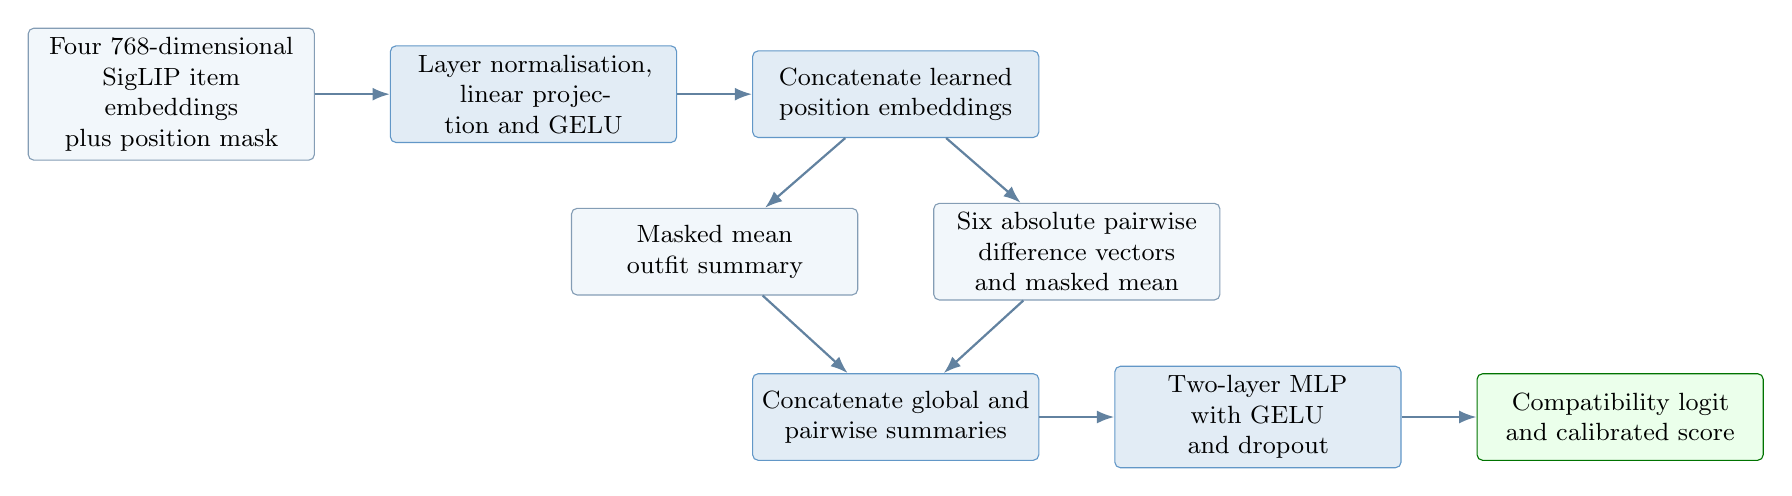
\begin{tikzpicture}[
    font=\small,
    box/.style={draw=wmgdarkblue!55, rounded corners=2pt, align=center,
      text width=34mm, minimum height=11mm, fill=wmgblue!6},
    key/.style={box, fill=wmgblue!14, draw=wmgblue!75},
    score/.style={box, fill=green!8, draw=green!45!black},
    arrow/.style={-{Latex[length=2.2mm]}, thick, draw=wmgdarkblue!70}
  ]
    \node[box] (input) at (0,3.2) {Four 768-dimensional\\SigLIP item embeddings\\plus position mask};
    \node[key] (projection) at (4.6,3.2) {Layer normalisation,\\linear projection and GELU};
    \node[key] (slots) at (9.2,3.2) {Concatenate learned\\position embeddings};

    \node[box] (pooled) at (6.9,1.2) {Masked mean\\outfit summary};
    \node[box] (pairs) at (11.5,1.2) {Six absolute pairwise\\difference vectors\\and masked mean};
    \node[key] (concat) at (9.2,-0.9) {Concatenate global and\\pairwise summaries};
    \node[key] (mlp) at (13.8,-0.9) {Two-layer MLP\\with GELU and dropout};
    \node[score] (logit) at (18.4,-0.9) {Compatibility logit\\and calibrated score};

    \draw[arrow] (input) -- (projection);
    \draw[arrow] (projection) -- (slots);
    \draw[arrow] (slots) -- (pairs);
    \draw[arrow] (slots) -- (pooled);
    \draw[arrow] (pairs) -- (concat);
    \draw[arrow] (pooled) -- (concat);
    \draw[arrow] (concat) -- (mlp);
    \draw[arrow] (mlp) -- (logit);
  \end{tikzpicture}}
  \caption{Architecture of the task-specific lightweight compatibility model}
  \label{fig:model-architecture}
\end{figure}


Training was limited to 12 epochs and used validation performance to select the
saved checkpoint. Three predefined random seeds were used to examine whether
results depended heavily on one training run. The test set was kept separate
from model selection.

The processed labels were already balanced, so the final model did not apply
additional positive-class weighting. Alternative weighting by outfit length
was tested but did not satisfy the complete acceptance criteria. The unweighted
model was therefore retained. Detailed settings and the rejected weighting
experiment are reserved for the appendices.

\section{Comparative experiments}

The proposed model was first compared with random ranking and a non-learned
SigLIP similarity baseline. These controls test whether the model performs
above chance and whether learning garment relationships adds value beyond the
frozen visual representation.

Three further models represented established directions in outfit-recommendation
research: a bidirectional LSTM based on \textcite{han2017bilstm}, a type-aware
pairwise model based on \textcite{vasileva2018typeaware}, and a
Transformer-based set model informed by \textcite{sarkar2023outfittransformer}.
They used the same processed data, frozen image representations and training
conditions as the proposed model. They are controlled implementations of the
main architectural ideas rather than exact reproductions of the published
systems.

Two ablation experiments were also conducted. One removed clothing-position
information, and the other removed the module that explicitly compares garment
pairs. The purpose was to determine whether these components made a measurable
contribution when the rest of the experimental conditions remained unchanged.

\section{Model and system evaluation}

Compatibility classification was evaluated using several complementary
measures. ROC--AUC measured how reliably positive outfits received higher
scores than negative outfits \parencite{fawcett2006roc}. Accuracy, balanced
accuracy, precision, recall, F1 and the confusion matrix were used to examine
classification behaviour at the selected threshold. Calibration measures were
reported separately because a model can rank examples correctly while still
producing overconfident scores \parencite{guo2017calibration}.

Recommendation performance was examined through the official fill-in-the-blank
task. One garment is removed from an outfit and the model must select the
correct replacement from four candidates. The correct answer was matched
through the outfit identifier because the answers in the disjoint data are
shuffled. Only questions compatible with the project's four clothing positions
were retained, and the retained proportion is reported with the result.

Confidence intervals were estimated by percentile bootstrap resampling
\parencite{efron1994bootstrap}. The selected-model AUC interval used 1,000
resamples of the 16,062 test rows; the selected FITB interval used 2,000
resamples of 4,468 retained questions. Structural-ablation intervals used
5,000 paired resamples of those questions after averaging correctness over the
three seeds. The exact-versus-quota score-loss interval used 2,000 resamples of
the 18 query-level differences. All reported intervals use the 2.5th and
97.5th percentiles. The same questions and random seeds
were used when comparing the complete model with an ablation, allowing their
differences to be assessed directly. Training, validation and test behaviour
were also compared to identify evidence of overfitting.

Expected calibration error used ten equal-width probability bins on the
validation examples. Scalar temperature scaling minimised validation binary
cross-entropy and did not use the test labels. Empty bins contributed no error;
each populated bin was weighted by its share of validation examples.

The complete application was tested separately from the classifier. Candidate
availability was checked under different weather and style conditions. Search
experiments examined whether the previous quota-based method could miss
higher-scoring combinations and measured the time required to search the
complete filtered candidate space.

Figure~\ref{fig:evaluation-framework} groups the evidence used to assess the
model and the surrounding recommendation process. No single metric is treated
as sufficient for deployment or for a claim about recommendation quality.

\begin{figure}[htbp]
  \centering
  \resizebox{\textwidth}{!}{%
  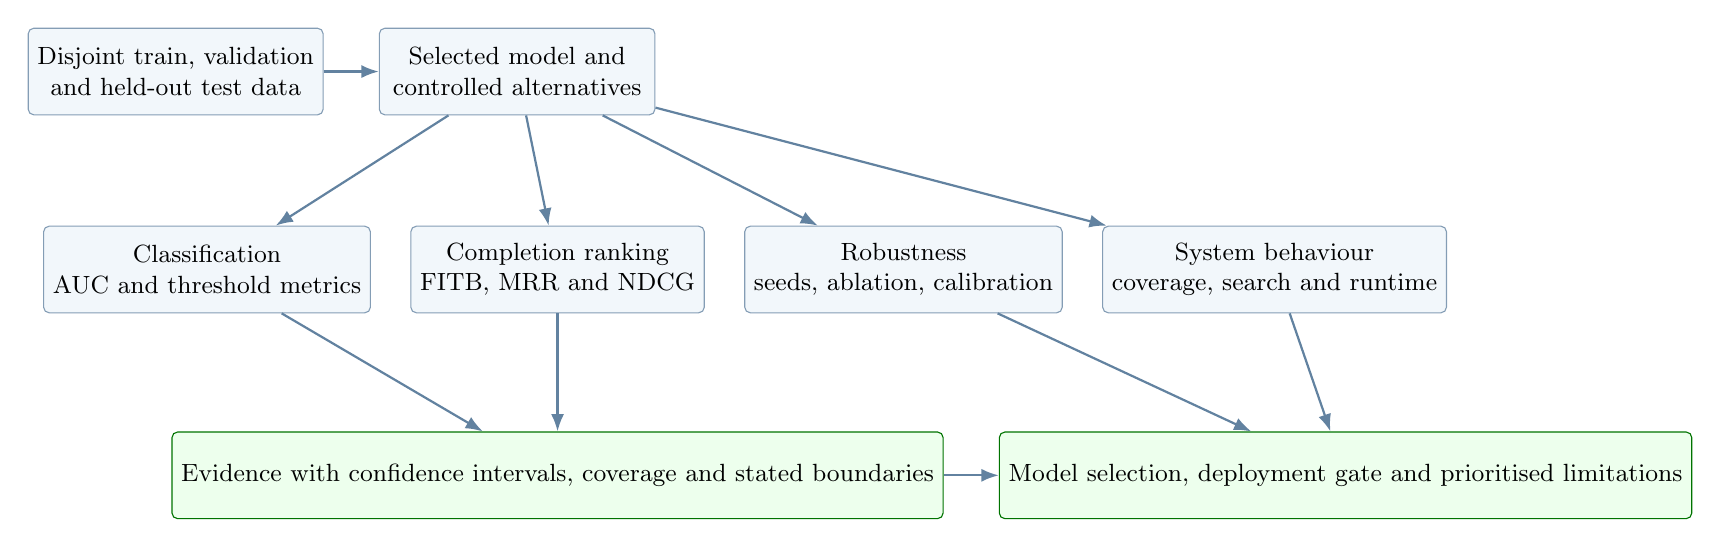
\begin{tikzpicture}[
    font=\small,
    box/.style={draw=wmgdarkblue!55, rounded corners=2pt, align=center,
      minimum width=35mm, minimum height=11mm, fill=wmgblue!6},
    evidence/.style={box, fill=green!7, draw=green!45!black},
    arrow/.style={-{Latex[length=2.2mm]}, thick, draw=wmgdarkblue!70}
  ]
    \node[box] (splits) {Disjoint train, validation\\and held-out test data};
    \node[box, right=7mm of splits] (model) {Selected model and\\controlled alternatives};

    \node[box, below left=14mm and 1mm of model] (classification) {Classification\\AUC and threshold metrics};
    \node[box, right=5mm of classification] (ranking) {Completion ranking\\FITB, MRR and NDCG};
    \node[box, right=5mm of ranking] (robustness) {Robustness\\seeds, ablation, calibration};
    \node[box, right=5mm of robustness] (system) {System behaviour\\coverage, search and runtime};

    \node[evidence, below=15mm of ranking] (claims) {Evidence with confidence intervals, coverage and stated boundaries};
    \node[evidence, right=7mm of claims] (decision) {Model selection, deployment gate and prioritised limitations};

    \draw[arrow] (splits) -- (model);
    \draw[arrow] (model) -- (classification);
    \draw[arrow] (model) -- (ranking);
    \draw[arrow] (model) -- (robustness);
    \draw[arrow] (model) -- (system);
    \draw[arrow] (classification) -- (claims);
    \draw[arrow] (ranking) -- (claims);
    \draw[arrow] (robustness) -- (decision);
    \draw[arrow] (system) -- (decision);
    \draw[arrow] (claims) -- (decision);
  \end{tikzpicture}}
  \caption{Evaluation framework connecting model, ranking and system evidence}
  \label{fig:evaluation-framework}
\end{figure}


\section{Experimental controls and decision rules}

The experiments were designed so that each comparison changed a defined part
of the pipeline. Architecture comparisons used the same processed examples,
frozen SigLIP features, epoch limit, optimiser settings and predefined random
seeds. This does not make the models identical in their learning behaviour,
but it reduces the risk that a reported difference is caused by one model
receiving different visual inputs or a more favourable data split. Parameter
counts and recorded training times were reported to place performance in the
context of model size and implementation cost. Training time was not treated
as a hardware-independent benchmark.

Model selection was separated from final reporting. Validation AUC selected
the saved checkpoint, and the test data were then used to estimate performance
on unseen examples. The three-seed architecture experiment examined variation
from initialisation and training order. Multiple runs cannot remove every
source of benchmark uncertainty. They provide more reliable evidence than one
favourable run \parencite{bouthillier2021variance}. Paired bootstrap
comparisons reused the same resampled test examples for the two models being
compared. This preserves the relationship between their predictions and is
more informative than treating the scores as unrelated observations
\parencite{dietterich1998tests,efron1994bootstrap}.

Decisions about model changes used more than overall AUC. The length-weighting
experiment had to retain overall discrimination, avoid reducing macro-level
performance and improve the weakest length group. It was rejected when the
weakest group deteriorated, despite a small improvement in overall mean AUC.
The ranking-loss experiment was also not adopted because it did not improve
the retained completion result. These decision rules reduce the temptation to
select a configuration from one favourable number after seeing the results.
They remain specific to the tested alternatives and do not imply that all
weighting or ranking losses are unsuitable.

The search comparison also kept the scoring objective and candidate artefact
fixed. Exact enumeration and quota-limited retrieval received the same held-out
inputs and feasible candidate states. The exact path supplied the reference
top results for the bounded space. Top-one recovery, top-ten recall, score loss
and runtime then described what the quota path gained and lost. A higher model
score was interpreted only as better optimisation of the deployed
compatibility objective.

The 18 inputs were a deterministic coverage sample rather than a random or
statistically representative sample. Positive examples in the processed
disjoint test split were pooled by occupied clothing position in their stored
order. The query index then cycled through all nine supported styles twice,
rotated the fixed input across the four clothing positions, and cycled through
the 12 interface colour labels. This produced five inner-top, five outer-layer,
four bottom and four shoe inputs. The recorded run used the womenswear candidate
range. Ground-truth garments from the held-out outfits were not inserted as
candidate answers, and the script applied no result-based filtering to the 18
generated cases. This sample supports a controlled engineering comparison of
the two search procedures; its size and deterministic construction limit wider
statistical generalisation.

\section{Application integration, bias and reproducibility}

The recommendation interface presents broad clothing concepts such as a black
casual jacket or white trainers rather than claiming that the model has
selected a particular commercial product. These concepts are derived from
garments in the Polyvore training split and are displayed as coloured icons.
Photographs are used only for garments uploaded or saved by the user.

Weather data were requested from the Open-Meteo forecast service
\parencite{openmeteo2026}. Weather, clothing position and the selected menswear
or womenswear range are treated as explicit constraints. The application does not infer gender from a
photograph. Because pure menswear training examples are limited, the same
compatibility model is used for both ranges and no claim is made that their
reliability is equal.

Reproducibility records include random seeds, model settings, training
histories, software versions, file hashes and evaluation outputs. Automated
tests cover data shapes, missing clothing positions, corrected fill-in-the-blank
labels, clothing-range filtering, recommendation determinism and search safety
limits. These records allow the reported experiments to be checked without
relying only on the running user interface.

The software was organised so that training, evaluation and application
inference could be run independently. Processed tensors and frozen embeddings
were stored as explicit artefacts, rather than being recreated silently during
each training run. Model checkpoints include the configuration required to
reconstruct the compatibility head, while evaluation scripts write structured
result files used by the tables in Chapter 4. This separation reduces the risk
that interface state or later UI changes alter a reported experiment.

Integration used a guarded loading path. The application first checks whether
the candidate artefact, model checkpoint and required metadata are present and
compatible. If they are available, the learned score participates in ranking;
otherwise the existing rule procedure is used and the fallback reason is
recorded. The model was not allowed to replace category, weather or
clothing-range validation. This design made it possible to test learned
recommendation without making the whole application dependent on one model
file. It also distinguishes reproducibility of an experimental checkpoint from
availability of a user-facing feature.

The runtime sequence is shown in Figure~\ref{fig:runtime-flow}. The selected
garment remains fixed, contextual constraints define the feasible candidate
space, and the learned model ranks complete combinations. A deterministic
content-based path is retained only as an operational fallback when the
required model artefacts cannot be loaded.

\begin{figure}[htbp]
  \centering
  \resizebox{\textwidth}{!}{%
  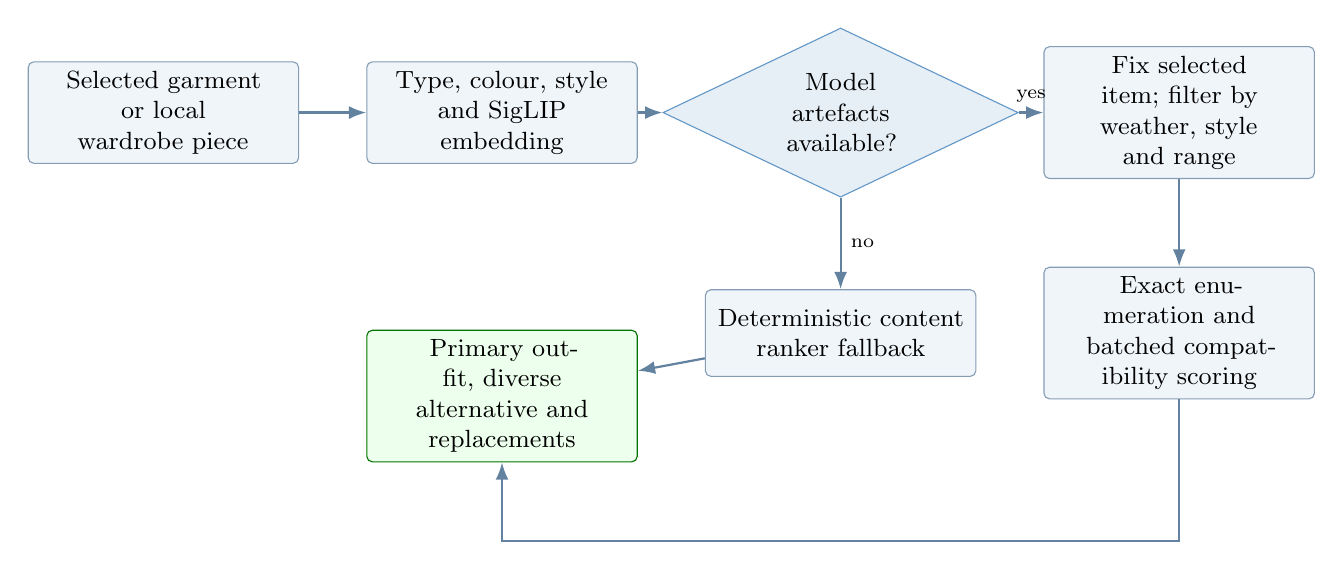
\begin{tikzpicture}[
    font=\small,
    flowbox/.style={draw=wmgdarkblue!55, rounded corners=2pt, align=center,
      text width=32mm, minimum height=11mm, fill=wmgblue!7},
    decision/.style={diamond, draw=wmgblue!75, align=center, aspect=2.1,
      text width=21mm, inner sep=1.5pt, fill=wmgblue!12},
    output/.style={flowbox, fill=green!7, draw=green!45!black},
    arrow/.style={-{Latex[length=2.2mm]}, thick, draw=wmgdarkblue!70}
  ]
    \node[flowbox] (image) at (0,2.4) {Selected garment\\or local wardrobe piece};
    \node[flowbox] (analyse) at (4.3,2.4) {Type, colour, style\\and SigLIP embedding};
    \node[decision] (available) at (8.6,2.4) {Model artefacts\\available?};
    \node[flowbox] (filter) at (12.9,2.4) {Fix selected item; filter by\\weather, style and range};
    \node[flowbox] (search) at (12.9,-0.4) {Exact enumeration and\\batched compatibility scoring};
    \node[flowbox] (fallback) at (8.6,-0.4) {Deterministic content\\ranker fallback};
    \node[output] (results) at (4.3,-1.2) {Primary outfit, diverse\\alternative and replacements};

    \draw[arrow] (image) -- (analyse);
    \draw[arrow] (analyse) -- (available);
    \draw[arrow] (available) -- node[above,font=\scriptsize]{yes} (filter);
    \draw[arrow] (filter) -- (search);
    \draw[arrow] (search.south) -- ++(0,-1.8) -| (results.south);
    \draw[arrow] (available) -- node[right,font=\scriptsize]{no} (fallback);
    \draw[arrow] (fallback) -- (results);
  \end{tikzpicture}}
  \caption{Runtime recommendation and fallback flow}
  \label{fig:runtime-flow}
\end{figure}


The interface was designed to make the main workflow easy to follow without
requiring knowledge of the underlying model. From the home page, the user can
set or select a saved city, choose a visual mood, and continue either by
starting with a garment or by opening the local wardrobe. In the recommendation
path, the user supplies and selects the garment region, chooses a style and a
menswear or womenswear candidate range, and then receives a ranked outfit with
alternatives. Pieces and completed outfits can subsequently be saved and
managed locally. Figure~\ref{fig:cove-home-interface} shows the implemented
entry point, including the weather scene, location controls, mood selector and
two principal actions.

\begin{figure}[htbp]
  \centering
  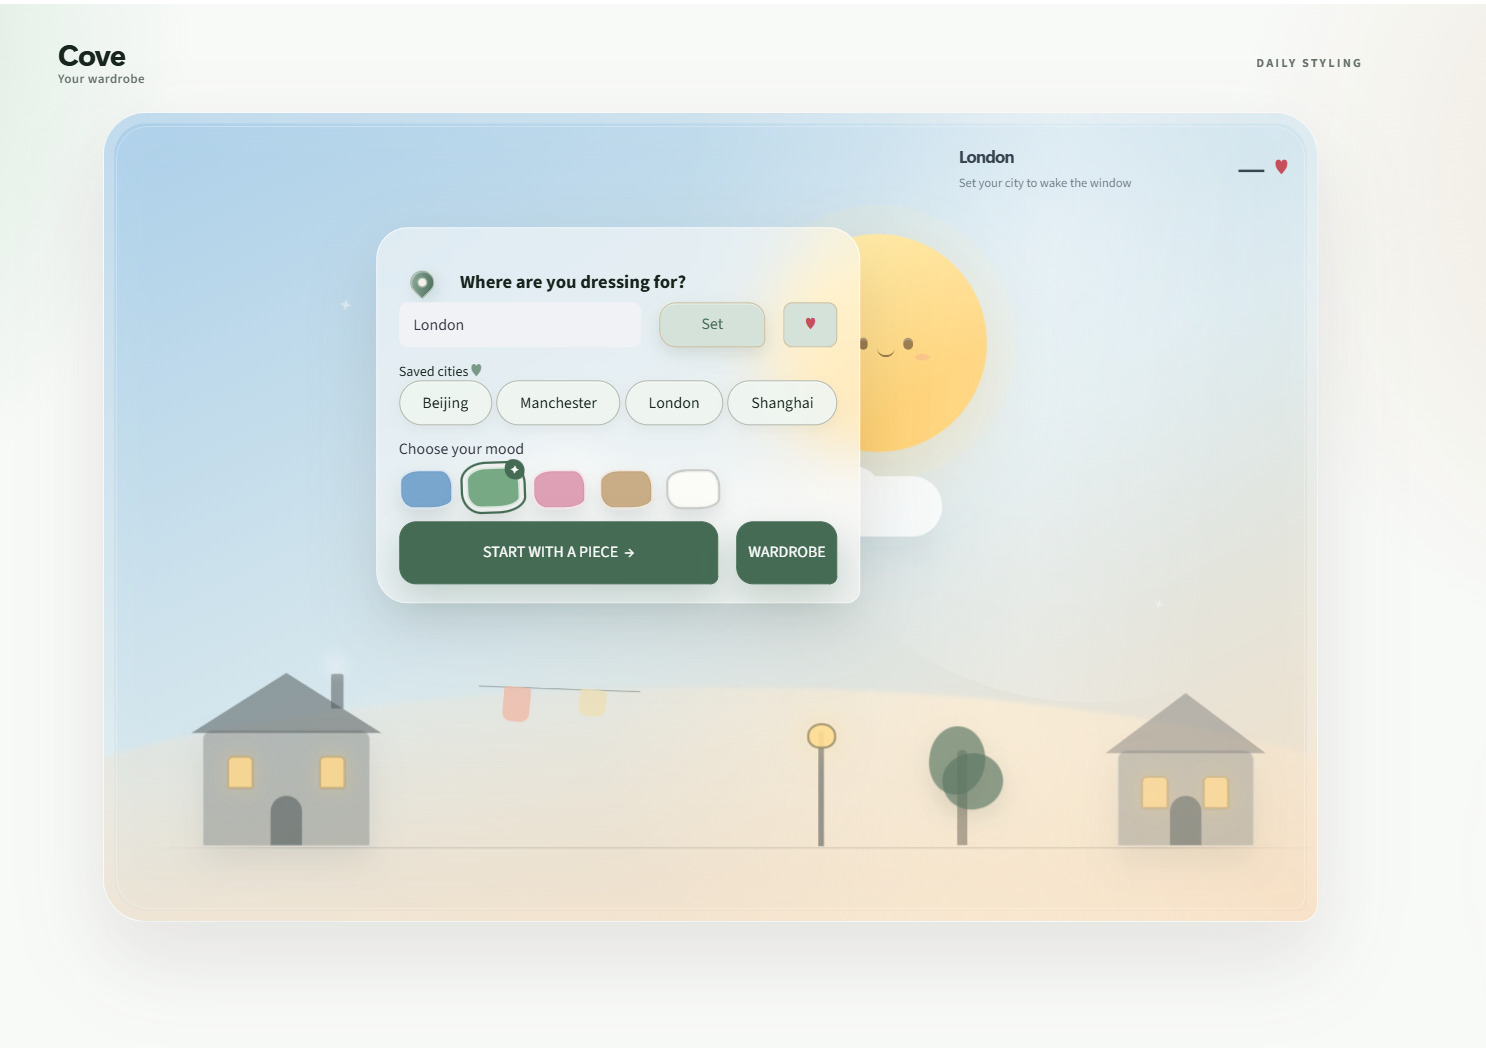
\includegraphics[width=0.94\textwidth]{assets/cove_homepage.png}
  \caption{Cove home interface showing the weather scene, location controls,
  mood selector and routes to garment selection and the local wardrobe}
  \label{fig:cove-home-interface}
\end{figure}

Visual hierarchy, large action controls and a short route to the two core tasks
were used to support a convenient and visually coherent interaction. Five soft
colour themes provide visual personalisation. The two-part clothing-range
control also keeps menswear and womenswear recommendations under direct user
control: the selected half is emphasised in the active theme colour, and the
system does not infer gender from the uploaded image. These features were
designed to support clear, accessible interaction. They
are not reported as measured usability results because no
participant evaluation was conducted.

Figure~\ref{fig:cove-recommendation-interface} shows the later stage of the
same journey. The selected garment remains visible beside the controls, the
chosen clothing range and style are explicit, and two complete outfit options
are presented with abstract coloured garment icons. The user can request a
model-ranked alternative for an individual position or save either complete
outfit. An optional designer-discovery panel illustrates how a future product
or independent-designer link could be added without changing the abstract
recommendation itself.

\begin{figure}[htbp]
  \centering
  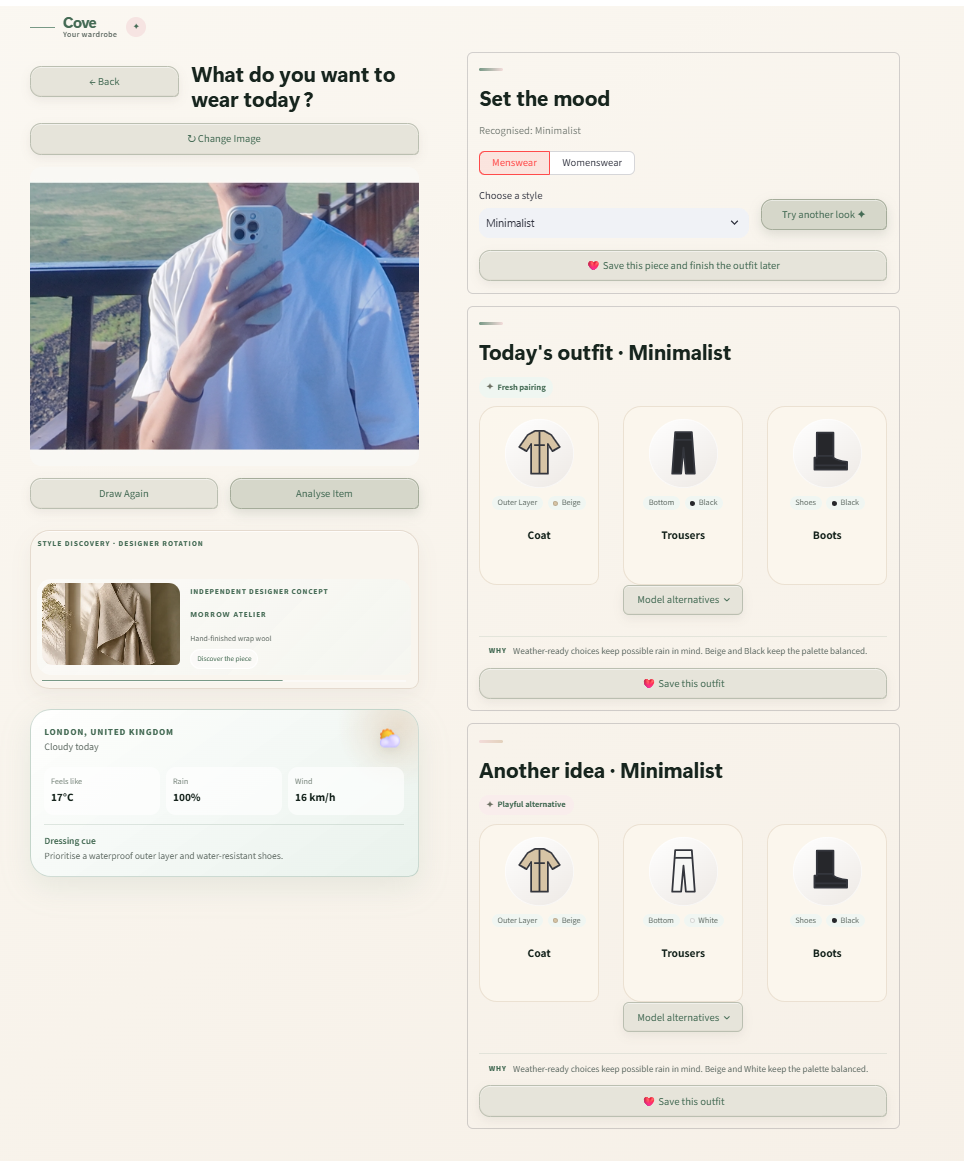
\includegraphics[width=0.82\textwidth]{assets/cove_recommendation.png}
  \caption{Cove recommendation interface showing the fixed garment, explicit
  clothing-range and style controls, abstract outfit alternatives and local
  save actions}
  \label{fig:cove-recommendation-interface}
\end{figure}

Table~\ref{tab:application-functions} records the responsibility of each core
application module. This division prevents the compatibility score from being
described as if it also performs recognition, weather validation or storage.

\begin{table}[htbp]
  \centering
  \caption{Core functions of the Cove prototype}
  \label{tab:application-functions}
  \small
  \begin{tabularx}{\textwidth}{@{}p{0.19\textwidth}p{0.25\textwidth}X@{}}
    \toprule
    \textbf{Module} & \textbf{Main input and output} & \textbf{Responsibility} \\
    \midrule
    Garment analysis & Selected crop $\rightarrow$ type, colour, style and embedding & Interprets the item supplied by the user and prepares its model representation. \\
    Candidate control & Context and fixed item $\rightarrow$ feasible states & Applies position, weather, style and clothing-range constraints. \\
    Compatibility ranking & Complete candidates $\rightarrow$ ordered scores & Scores relational coherence using the small project-specific head. \\
    Wardrobe management & Piece and outfit edits $\rightarrow$ local records and images & Saves, reuses, renames, groups and removes local wardrobe content. \\
    Fallback & Recognised item and context $\rightarrow$ rule-ranked outfit & Preserves basic operation when learned artefacts are absent or incompatible. \\
    \bottomrule
  \end{tabularx}
\end{table}

Persistent state is implemented through JSON documents and local image files,
while model and research outputs remain separate artefacts.
Figure~\ref{fig:local-data-relationships} presents these
logical relationships without implying tables, foreign keys or a database
engine that are not present in the implementation.

\begin{figure}[htbp]
  \centering
  \resizebox{\textwidth}{!}{%
  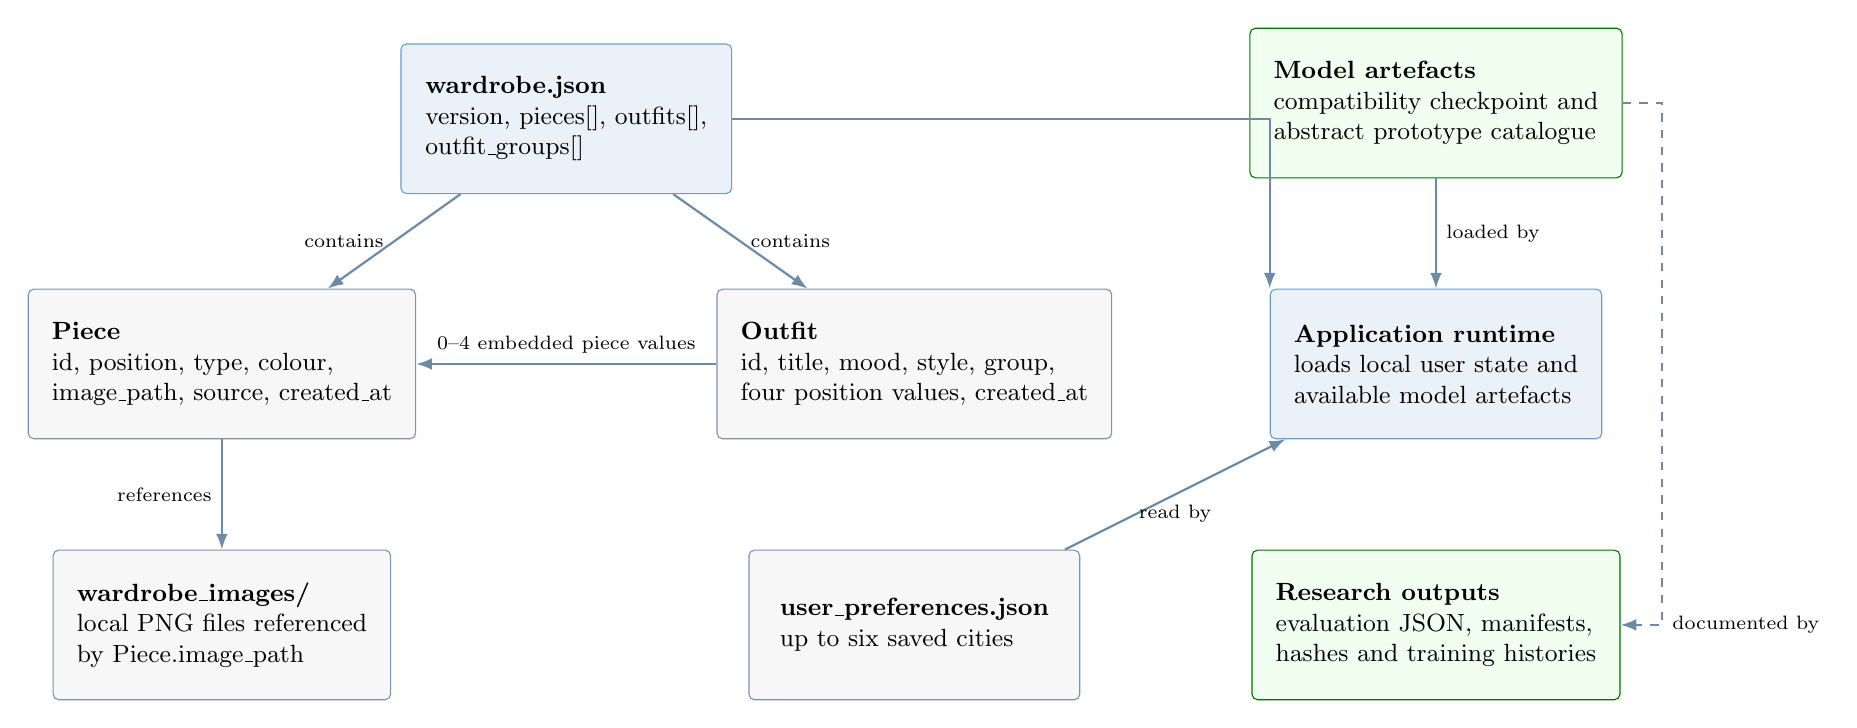
\begin{tikzpicture}[
    font=\small,
    entity/.style={draw=wmgdarkblue!60, rounded corners=2pt, align=left,
      minimum width=42mm, minimum height=19mm, fill=gray!6, inner sep=3mm},
    store/.style={entity, fill=wmgblue!10, draw=wmgblue!70},
    artefact/.style={entity, fill=green!6, draw=green!45!black},
    rel/.style={-{Latex[length=2mm]}, thick, draw=wmgdarkblue!65}
  ]
    \node[store] (wardrobe) {\textbf{wardrobe.json}\\version, pieces[], outfits[],\\outfit\_groups[]};
    \node[entity, below left=12mm and -2mm of wardrobe] (piece) {\textbf{Piece}\\id, position, type, colour,\\image\_path, source, created\_at};
    \node[entity, below right=12mm and -2mm of wardrobe] (outfit) {\textbf{Outfit}\\id, title, mood, style, group,\\four position values, created\_at};
    \node[entity, below=14mm of piece] (images) {\textbf{wardrobe\_images/}\\local PNG files referenced\\by Piece.image\_path};
    \node[entity, below=14mm of outfit] (prefs) {\textbf{user\_preferences.json}\\up to six saved cities};
    \node[store, right=20mm of outfit] (runtime) {\textbf{Application runtime}\\loads local user state and\\available model artefacts};
    \node[artefact, above=14mm of runtime] (model) {\textbf{Model artefacts}\\compatibility checkpoint and\\abstract prototype catalogue};
    \node[artefact, below=14mm of runtime] (results) {\textbf{Research outputs}\\evaluation JSON, manifests,\\hashes and training histories};

    \draw[rel] (wardrobe) -- node[left,font=\scriptsize]{contains} (piece);
    \draw[rel] (wardrobe) -- node[right,font=\scriptsize]{contains} (outfit);
    \draw[rel] (outfit) -- node[above,font=\scriptsize]{0--4 embedded piece values} (piece);
    \draw[rel] (piece) -- node[left,font=\scriptsize]{references} (images);
    \draw[rel] (wardrobe.east) -| (runtime.north west);
    \draw[rel] (prefs) -- node[below,font=\scriptsize]{read by} (runtime);
    \draw[rel] (model) -- node[right,font=\scriptsize]{loaded by} (runtime);
    \draw[rel,dashed] (model.east) -- ++(5mm,0) |- node[right,font=\scriptsize]{documented by} (results.east);
  \end{tikzpicture}}
  \caption{Logical relationships among local user data and model artefacts; the prototype uses files rather than a relational database}
  \label{fig:local-data-relationships}
\end{figure}


\begin{table}[htbp]
  \centering
  \caption{Local persistence and research artefacts}
  \label{tab:local-persistence}
  \small
  \begin{tabularx}{\textwidth}{@{}p{0.27\textwidth}p{0.27\textwidth}X@{}}
    \toprule
    \textbf{File or artefact} & \textbf{Principal contents} & \textbf{Role and relationship} \\
    \midrule
    \texttt{wardrobe.json} & Pieces, outfits and outfit groups & Local user store; each outfit contains values for the four supported positions. \\
    \texttt{wardrobe\_images/} & User garment PNG files & Image paths are referenced by saved piece records. \\
    \texttt{user\_preferences.json} & Saved cities & Read by the application to restore local location choices. \\
    Compatibility checkpoint & Model configuration, state and metadata & Reconstructs the selected compatibility scorer at runtime. \\
    Abstract prototype artefact & Candidate states and frozen embeddings & Supplies the product-independent candidate space for constrained search. \\
    Evaluation JSON and manifests & Metrics, histories, hashes and settings & Preserve the evidence chain; they are not user-profile records. \\
    \bottomrule
  \end{tabularx}
\end{table}

Supplementary software-design views are provided in
Appendix~\ref{app:software-design}. They include the implemented use cases,
overall component structure, recommendation-module dependencies, a logical
entity-relationship view and traceable user stories. The diagrams describe the
current prototype rather than an assumed enterprise architecture.

Result artefacts and checkpoints are larger than ordinary source files and may
not always be suitable for repository distribution. File hashes and documented
generation commands therefore provide an additional check that a locally held
artefact corresponds to the evaluated version. This approach does not replace
archival storage or full environment preservation, but it provides a practical
chain from processed data to training history, evaluation output and deployed
configuration.

\section{Research risks and mitigation}

The investigation involved data, methodological, ethical and operational
risks. These were considered during development rather than being listed only
after the experiments. The first concerned data provenance and permitted use.
The project therefore used documented secondary datasets and kept their roles
separate. Polyvore supplied compatibility labels, whereas Zara was limited to
recognition and feature-domain diagnostics. User photographs remained local
and were not incorporated into the research dataset. Any later public release would require a separate
check before third-party images or large derived artefacts could be
redistributed.

Dataset availability was not treated as blanket permission to redistribute
third-party content. The public-code package should exclude source dataset
images, item-level embeddings and catalogue artefacts. The compact learned-head
checkpoints contain model tensors, configuration and training metadata rather
than source images or product identifiers; their redistribution should still
be covered by a separate licence review before public release. This distinction
keeps the ethical approval boundary, research use and publication permission
from being treated as interchangeable.

A second risk was data leakage. Product overlap between training and test data
could allow a model to recognise garments seen during training instead of
learning relationships that transfer to unseen items. The published split was
used to reduce this risk, and candidate concepts were derived from the training
division rather than the test division. The local identifier audit confirmed
zero outfit-ID overlap but found the residual item-ID overlaps reported above,
so strict item-level separation cannot be claimed. Model selection and
temperature scaling used validation data, while the test set was reserved for
final evaluation. Repeatedly changing the model after inspecting test results
could still weaken test independence. The current test results are therefore
treated as final evidence for the selected model rather than as a further
tuning target.

The labels create a further interpretive risk. Positive examples are observed
Polyvore outfits, whereas negatives are constructed by replacing an item
within a broad category. A constructed negative is not proof that an outfit is
inherently unacceptable; it is a reproducible device for learning distinctions
within this dataset. Similarly, official FITB evaluation was restricted to
questions represented by the four supported positions and available
embeddings. Coverage is reported with accuracy so that performance on the
retained subset is not presented as a complete benchmark result. This follows
the principle that recommender metrics must be interpreted in relation to the
task and sampling protocol \parencite{herlocker2004evaluation}.

Overfitting and unstable model selection were addressed by recording training,
validation and test behaviour separately, using three random seeds for the
controlled architecture comparison and selecting checkpoints from validation
AUC. Confidence intervals were estimated for the principal test and paired
comparisons. Early stopping limits continued fitting after validation
performance stops improving, but does not remove a generalisation gap
\parencite{prechelt1998early}. The results therefore report both the close
validation--test result and the larger train--test difference.

Representation across clothing ranges was unequal. The retained FITB questions
and pure training examples were concentrated in womenswear, so the small
menswear subgroup could not support a reliable fairness comparison. The
interface asks users to choose a clothing range and does not infer gender from
an image. Menswear evidence is reported as sparse coverage rather than proof of
equal reliability. This does not resolve representational bias, but it avoids
automated gender classification and makes the evidential boundary explicit
\parencite{keyes2018misgendering,mehrabi2021bias}.

Finally, the deployed process could fail if model files, embeddings or
candidate records were unavailable, or if constraints removed every candidate
for a position. Release checks, deterministic seeds and recorded artefact paths
support reproducibility. Slot, weather and clothing-range constraints reject
infeasible combinations, while a deterministic rule-based fallback allows the
application to continue when learned artefacts cannot be loaded. These mitigations make failure conditions more
visible and bounded, without implying that technical testing removes all
social or external-validity risks.

\section{Summary}

The methodology combines a frozen visual encoder, a small project-specific
compatibility head and a constrained recommendation process. Controlled baselines, repeated
training runs, fill-in-the-blank evaluation, ablation experiments and system
tests were used to examine different aspects of performance. The following
chapter reports the corresponding results.

\chapter{Results}

\section{Introduction}

This chapter reports the compatibility, architecture, ablation, overfitting,
bias and candidate-search results. Results are separated according to their
experimental protocol. In particular, the selected compatibility model, the
three-seed architecture comparison and the candidate-search experiment are
reported independently because they answer different questions.

\section{Selected compatibility-model performance}

The selected compatibility model was evaluated on 16,062 held-out test
examples containing equal numbers of positive and negative rows. It achieved a
test ROC--AUC of 0.8583, with a 95\% confidence interval from 0.8524 to 0.8641.
Accuracy and balanced accuracy were both 0.7664. \Cref{tab:final-model-results}
reports the remaining classification results.

\begin{table}[htbp]
  \centering
  \caption{Held-out performance of the selected compatibility model}
  \label{tab:final-model-results}
  \begin{tabular}{lr}
    \toprule
    Metric & Result \\
    \midrule
    ROC--AUC & 0.8583 \\
    95\% AUC confidence interval & 0.8524--0.8641 \\
    Average precision & 0.8558 \\
    Accuracy & 0.7664 \\
    Balanced accuracy & 0.7664 \\
    Precision & 0.7240 \\
    Recall & 0.8610 \\
    F1 & 0.7866 \\
    Specificity & 0.6718 \\
    Matthews correlation coefficient & 0.5426 \\
    Brier score & 0.1599 \\
    \bottomrule
  \end{tabular}
\end{table}

At the 0.5 threshold, the model correctly classified 5,395 negative and 6,915
positive outfits. It classified 2,636 negative outfits as positive and 1,116
positive outfits as negative. Recall was therefore higher than specificity at
this threshold.

A separate fixed-seed baseline experiment produced an AUC of 0.4940 for
deterministic random scores and 0.7012 for mean pairwise SigLIP cosine
similarity. The learned head in that experiment reached 0.8573. These values
came from an earlier controlled baseline run and are reported separately from
the selected model result of 0.8583. A mean-pooled frozen-SigLIP logistic
baseline, evaluated on the same processed test rows, reached AUC 0.5532. Its
deterministic preprocessing produced the same value in the three recorded seed
files.

\section{Controlled architecture comparison}

Each learned architecture was trained with seeds 42, 7 and 123. The proposed
model achieved the highest mean test AUC and the smallest AUC standard deviation
across the three runs (\Cref{tab:architecture-results}).

\begin{table}[htbp]
  \centering
  \caption{Controlled three-seed architecture comparison}
  \label{tab:architecture-results}
  \begin{tabularx}{\textwidth}{>{\raggedright\arraybackslash}Xrrrr}
    \toprule
    Model & Parameters & Time (s) & Mean AUC & SD \\
    \midrule
    Bidirectional LSTM & 397,185 & 96.87 & 0.7928 & 0.0060 \\
    Type-aware pairwise & 591,489 & 7.99 & 0.7918 & 0.0129 \\
    Set Transformer & 374,145 & 7.03 & 0.7744 & 0.0133 \\
    Proposed model & 379,265 & 4.81 & 0.8596 & 0.0009 \\
    \bottomrule
  \end{tabularx}
\end{table}

The proposed model's mean balanced accuracy was 0.7742 and its mean Matthews
correlation coefficient was 0.5510. Mean balanced accuracy was 0.7138 for the
bidirectional LSTM, 0.7176 for the type-aware model and 0.7034 for the set
Transformer.

Paired bootstrap comparison of the three-seed mean predictions gave an AUC
difference of 0.0700 between the proposed model and the bidirectional LSTM
(95\% interval 0.0650--0.0753). The difference from the type-aware model was
0.0634 (0.0578--0.0694), while the difference from the set Transformer was
0.0801 (0.0750--0.0858). These results compare controlled implementations on
the project's processed data rather than the headline results in the original
publications.

\section{Fill-in-the-blank and ablation results}

Of 15,145 official disjoint FITB questions, 4,468 were compatible with the
project's four-position representation, giving coverage of 29.50\%. Other
questions were excluded because of unsupported answer positions, insufficient
supported garments, duplicate positions or an answer position already occupied
in the question.

The selected model achieved FITB accuracy of 0.6025. Its 95\% bootstrap
confidence interval was 0.5873--0.6175, compared with chance accuracy of 0.25.
Mean reciprocal rank was 0.7705 and normalised discounted cumulative gain was
0.8289.

The structural ablation used the same 4,468 questions and three random seeds.
The 0.6025 result above belongs to the selected seed-42 checkpoint; the complete
model row below is the mean of three separately retrained seed runs and is
therefore 0.5994.
\Cref{tab:ablation-results} reports the mean accuracy and the paired difference
between the complete model and each reduced variant.

\begin{table}[htbp]
  \centering
  \caption{Structural ablation on the retained official FITB subset}
  \label{tab:ablation-results}
  \begin{tabularx}{\textwidth}{>{\raggedright\arraybackslash}Xrrr}
    \toprule
    Configuration & Mean accuracy & Full minus variant & Paired 95\% interval \\
    \midrule
    Complete model & 0.5994 & --- & --- \\
    Without clothing-position embedding & 0.5947 & 0.0047 & -0.0013--0.0106 \\
    Without pairwise module & 0.4966 & 0.1028 & 0.0896--0.1157 \\
    \bottomrule
  \end{tabularx}
\end{table}

The retained FITB data contained only 46 menswear questions, compared with
4,422 womenswear questions. Menswear performance was therefore recorded as a
coverage limitation rather than treated as a reliable comparison between
clothing ranges. The descriptive subgroup values are provided in the
appendices.

\section{Calibration and overfitting audit}

The selected checkpoint reached its highest validation AUC at epoch 6. Training,
validation and test AUC were 0.9699, 0.8598 and 0.8583 respectively
(\Cref{tab:split-results}).

\begin{table}[htbp]
  \centering
  \caption{Performance of the selected checkpoint by data split}
  \label{tab:split-results}
  \begin{tabular}{lrrrr}
    \toprule
    Split & Examples & AUC & Accuracy & F1 \\
    \midrule
    Training & 18,243 & 0.9699 & 0.8997 & 0.9051 \\
    Validation & 3,274 & 0.8598 & 0.7688 & 0.7845 \\
    Test & 16,062 & 0.8583 & 0.7664 & 0.7866 \\
    \bottomrule
  \end{tabular}
\end{table}

The train--test AUC difference was 0.1116, while the absolute
validation--test difference was 0.00145. Validation AUC declined by 0.0100
between the saved epoch and the last observed epoch.

Validation-only temperature scaling produced a temperature of 1.5760.
Validation negative log-likelihood decreased from 0.5081 to 0.4776, while
expected calibration error decreased from 0.0772 to 0.0588. Candidate ordering
was unchanged by the calibration step. Expected calibration error used ten
equal-width probability bins over the 3,274 validation examples.

\section{Outfit-length imbalance and feature-domain results}

The class labels were balanced. A separate experiment examined the imbalance
between three-item and four-item outfits. \Cref{tab:length-weighting-results}
reports the three configurations across the same three seeds.

\begin{table}[htbp]
  \centering
  \caption{Outfit-length weighting experiment}
  \label{tab:length-weighting-results}
  \begin{tabularx}{\textwidth}{>{\raggedright\arraybackslash}Xrrr}
    \toprule
    Configuration & Overall AUC & Weakest-length AUC & Group gap \\
    \midrule
    Unweighted & 0.8596 & 0.8507 & 0.0393 \\
    Moderate length weighting & 0.8601 & 0.8500 & 0.0433 \\
    Stronger length weighting & 0.8553 & 0.8438 & 0.0485 \\
    \bottomrule
  \end{tabularx}
\end{table}

Moderate weighting achieved the highest overall mean AUC but reduced the mean
result for the weakest length group and increased the group gap. It therefore
failed the predefined deployment gate, and the unweighted configuration was
retained.

The feature-domain diagnostic compared 26,124 Polyvore test items with 300 Zara
catalogue items. The domain classifier achieved cross-validated AUC of 1.000.
Centroid cosine similarity was 0.7452, and the mean nearest-Polyvore similarity
for the Zara items was 0.6528. The implications of this separability are
considered in Chapter 5.

\section{Candidate-search results}

The product-independent candidate artefact contained 1,670 clothing concepts
derived from the Polyvore training split, covering 23 garment types, 12 colours
and nine styles. The selected womenswear range contained 1,508 concepts and the
menswear range contained 162. Both ranges contained candidates for all four
supported clothing positions.

The earlier retailer-derived candidate space contained 300 product records and
122 visible type--colour combinations. The product-independent representation
contained 271 such combinations. Absolute compatibility scores across these
candidate sources were not treated as directly comparable because their data
distributions differ.

Exact and quota-limited search were compared on 18 held-out inputs using the
same product-independent candidate space and compatibility model. The
quota-limited path recovered the exact top result in 27.78\% of queries and had
mean recall of 24.44\% for the exact top ten. It examined a mean 3.41\% of the
candidate combinations.

The mean score loss relative to the highest score found by exact search was
0.0179, with a 95\% bootstrap interval of 0.0063--0.0357. Thirteen of the 18
queries had a positive score loss. Repeated exact searches returned the same
top-ten results for every tested query.

\begin{table}[htbp]
  \centering
  \caption{Exact-search and quota-limited search results}
  \label{tab:search-results}
  \begin{tabular}{lr}
    \toprule
    Measure & Quota-limited result \\
    \midrule
    Exact top result recovered & 27.78\% \\
    Mean recall of exact top ten & 24.44\% \\
    Mean candidate space examined & 3.41\% \\
    Mean score loss & 0.0179 \\
    Queries with positive score loss & 13 of 18 \\
    \bottomrule
  \end{tabular}
\end{table}

On the recorded CPU experiment, exact search had a median runtime of 0.474
seconds, a 95th-percentile runtime of 2.107 seconds and a maximum of 3.206
seconds. Quota-limited search over the same candidate space had a median runtime
of 0.028 seconds.

Candidate availability was tested across four weather scenarios and nine
styles, giving 36 combinations. Every tested combination retained all four
logical clothing positions. In hot-weather cases, the outer-layer position was
represented by the explicit masked \emph{No Outer Layer} option.

\section{Summary}

The selected compatibility model achieved test AUC of 0.8583 and FITB accuracy
of 0.6025 on the retained official subset. The three-seed comparison recorded a
higher mean AUC for the proposed architecture than for the three controlled
learned baselines. Removing the pairwise module produced a clear reduction,
whereas the interval for removing clothing-position information crossed zero.

The selected model showed a substantial train--test gap but close validation
and test performance. Validation-only calibration reduced negative
log-likelihood and expected calibration error. The tested outfit-length
weighting did not pass its deployment gate.

The product-independent candidate representation expanded the range of visible
type--colour combinations. The quota-limited search recovered the same highest
scoring result as exact search in 27.78\% of the tested queries while requiring
substantially less runtime. Chapter 5 examines the meaning and limitations of
these results.

\chapter{Analysis}

\section{Introduction}

This chapter analyses what can reasonably be concluded from the results in
Chapter 4. It considers the evidence provided by the controlled baselines,
structural ablations, generalisation audit and candidate-search experiment. It
also distinguishes results that support the proposed design from those that
reveal uncertainty or limitations.

The analysis remains within the scope of the experiments. A model score
represents compatibility learned from the processed Polyvore data. It does not
measure whether an individual user likes an outfit, whether the outfit is
objectively fashionable or whether a recommended concept will lead to a
purchase.

\section{Compatibility performance and baseline evidence}

The selected compatibility model achieved an AUC of 0.8583 on the held-out
test data. This means that the model usually assigned a higher score to a
randomly selected positive outfit than to a randomly selected negative outfit
\parencite{fawcett2006roc}. It does not mean that 85.83\% of recommendations are
correct or will be liked by users.

The non-learned SigLIP similarity baseline reached an AUC of 0.7012. Frozen
visual features therefore contained some information related to the dataset
labels without compatibility training. The learned model nevertheless
performed substantially better under the same processed test protocol. This
difference supports the need to learn relationships among garments rather than
relying only on general visual similarity, consistent with the distinction
between similarity and complementarity made by \textcite{mcauley2015styles}.

The proposed architecture also exceeded the three controlled learned baselines
across the predefined seeds. Paired AUC intervals remained above zero for the
comparisons with the bidirectional LSTM, type-aware model and set Transformer.
Within this experiment, the result was therefore not produced by one favourable
initialisation or one unusually weak baseline run.

This does not demonstrate that the proposed model is universally superior to
the published architectures. The comparison models were controlled adaptations
using frozen SigLIP inputs and the project's four-position representation. The
evidence shows that, under these shared conditions, the lightweight design was
more effective than the selected alternatives. Direct comparison with published
headline values would not be valid because the encoders, filtering and test
coverage differ.

The proposed model was also the fastest of the four learned architectures in
the recorded training experiment. This supports its description as lightweight
within the project. The timing remains dependent on the implementation,
hardware and frozen-input pipeline and is not a universal speed comparison.

\section{Architectural evidence}

Removing the pairwise module reduced mean FITB accuracy by 10.28 percentage
points. The paired confidence interval remained entirely above zero. This
provides the clearest structural evidence in the study: explicitly comparing
garments contributed information that was not recovered by the overall outfit
summary alone.

The finding accords with the relational treatment of compatibility in earlier
work \parencite{vasileva2018typeaware,sarkar2023outfittransformer}. A garment
may be plausible in one combination but not another, so an average outfit
representation can lose differences between particular items. The pairwise
component preserves a summary of these relationships without requiring a much
larger attention model. This is evidence about the tested implementation rather
than proof that pairwise aggregation is always preferable to attention.

Removing clothing-position information produced only a small reduction, and
its confidence interval crossed zero. The experiment therefore does not provide
clear evidence that the position embedding improved FITB performance. One
possible explanation is that the visual representation and pairwise relations
already contain information that distinguishes broad garment roles. This is a
possible explanation rather than a demonstrated cause.

The position embedding was retained because it adds little computational cost
and gives the model an explicit indication of clothing role. Nevertheless, it
should not be described as an empirically necessary component. A simpler model
without it remains a reasonable alternative for future evaluation.

\section{Generalisation, overfitting and calibration}

Training AUC of 0.9699 was considerably higher than test AUC of 0.8583. The
difference shows that the model fitted the training data more strongly than it
generalised to unseen examples. The results therefore contain evidence of
training-set overfitting.

Validation and test AUC differed by only 0.00145, and the saved checkpoint
corresponded to the highest observed validation AUC. Validation-based checkpoint
selection therefore behaved consistently on the held-out test split. It does
not remove the train--test gap, but continuing beyond the selected epoch was not
supported by the validation results. This is the limited role expected of early
stopping: it controls continued fitting after validation performance peaks but
does not guarantee the absence of overfitting \parencite{prechelt1998early}.

Further tuning against the current test results would weaken the independence of
the test set. Additional regularisation experiments should therefore use
validation-only decisions or introduce a new untouched evaluation split. The
current checkpoint is a more defensible stopping point than repeatedly changing
the model after inspecting its test performance.

Temperature scaling reduced validation negative log-likelihood and expected
calibration error. The original scores were therefore more confident than
necessary on the validation data. Calibration improves the interpretation of
confidence but does not alter recommendation order or provide evidence of
improved compatibility ranking \parencite{guo2017calibration}.

\section{Outfit-length imbalance}

The dataset was balanced between positive and negative labels, so the principal
imbalance did not concern class counts. Instead, three-item outfits were more
common than four-item outfits. Moderate length weighting produced a slightly
higher overall mean AUC but reduced performance for the weakest length group and
increased the difference between the two groups.

Selecting that configuration only because its overall AUC was marginally higher
would conflict with the purpose of the weighting experiment. The predefined
gate required the weakest group to improve rather than allowing a small overall
gain to hide weaker group performance. Retaining the unweighted configuration
was therefore consistent with the stated decision rule.

This result does not show that weighting can never improve the model. It shows
only that the tested schemes did not provide a sufficiently balanced improvement
under the present data and acceptance criteria.

\section{Relationship between learned scores and explicit constraints}

The application does not allow the compatibility score to decide every part of
an outfit. This separation is necessary because statistical compatibility and
feasibility answer different questions. The model estimates whether a complete
combination resembles compatible relationships in the processed training data.
It does not know that an outer layer may be unnecessary in hot weather, that a
user-selected garment must remain fixed, or that a candidate belongs to the
requested clothing range. These conditions are applied before or during search
rather than learned indirectly from the score.

The arrangement has two analytical advantages. First, a recommendation can be
traced through candidate construction, constraint filtering and final scoring.
If no outer layer is shown, the system can identify a weather mask rather than
attribute the decision vaguely to the neural model. If an unsuitable clothing
range appears, the error lies in filtering or metadata rather than in the
compatibility score. This is a limited form of procedural explanation: it does
not explain the visual features learned by SigLIP, but it identifies which
system component made a deterministic decision.

Second, the rules stop the model from being evaluated for knowledge that its
training objective did not provide. A positive or negative outfit label does
not directly encode local weather, personal wardrobe ownership or application
state. Expecting the compatibility head to infer these factors would mix
separate sources of evidence and make failures harder to diagnose. The modular
design therefore supports auditability even though it may be less flexible
than one end-to-end model.

This division also creates limitations. A rule can exclude a combination that
the model would score highly, and errors in garment metadata can remove valid
candidates before ranking. The reported model AUC does not test those rule
failures. For this reason, model evaluation and 36-case candidate-availability
testing were reported separately. The deterministic fallback is handled in the
same way. It keeps the application usable when model artefacts are absent, but
its output should not be combined with learned-model results or described as
equivalent in quality.

\section{Candidate-search completeness and latency}

Quota-limited search examined an average of 3.41\% of the feasible combinations.
It recovered the same highest-scoring result as exact search in 27.78\% of 18
queries and recovered an average of 24.44\% of the exact top ten. The quota
stage therefore frequently removed combinations that the compatibility model
would otherwise have ranked highly.

A positive score loss in 13 of the 18 queries confirms that the change was not
limited to rearranging equally scored candidates. Score loss refers only to the
deployed model objective, however; it does not establish that a person would
prefer the exact-search result.

Exact search increased median runtime from approximately 0.028 seconds to 0.474
seconds on the recorded CPU experiment. Its 95th-percentile runtime remained
close to two seconds. The experiment identifies a clear trade-off: exact search
provides completeness under the model objective, while quota search provides
lower latency. This reflects the broader retrieval trade-off between search
coverage and computational cost \parencite{johnson2021similarity}.

Within the tested candidate sizes, the additional runtime remained compatible
with an interactive prototype. This statement applies only to the recorded
hardware and bounded search space. A substantially larger catalogue could
require approximate retrieval, staged ranking or another search strategy.

\section{Coverage, domain shift and bias limitations}

Only 29.50\% of the official FITB questions could be represented by the four
supported clothing positions. The resulting FITB accuracy is valid only for the
retained subset and cannot be presented as performance on the complete official
benchmark.

Menswear evidence was particularly sparse. Only 46 retained FITB questions
were labelled as menswear, and the training data contained very few purely
menswear outfits. The figures identify a coverage problem but do not estimate a
dependable performance difference between clothing ranges.

The feature-domain classifier separated Polyvore and Zara items with an AUC of
1.000. Their frozen feature distributions were therefore distinguishable under
the diagnostic procedure. This does not measure how much compatibility accuracy
would decline on Zara because compatible Zara outfit labels were unavailable.
The result instead prevents an unsupported assumption that performance transfers
unchanged between the two sources.

The candidate system avoids presenting historical product brands and allows the
user to choose a clothing range, retain the uploaded garment and reject
alternatives. These choices improve control and reduce some immediate product
risks, but they do not remove bias inherited from Polyvore labels or the frozen
visual representation \parencite{mehrabi2021bias,selbst2019fairness}.

Finally, no participant evidence is available. The project can support claims
about offline compatibility discrimination, candidate completion, search
completeness and system behaviour. It cannot establish emotional benefit, trust,
usability across populations or preference improvement.

\section{Summary}

The strongest model evidence comes from the controlled architecture comparison
and removal of the pairwise module. Together, these results support a lightweight
relational head on frozen visual representations within the processed Polyvore
task. Evidence for the clothing-position embedding is inconclusive.

The selected checkpoint retains an overfitting tendency, although
validation-based selection produced closely aligned validation and test results.
Calibration improved validation confidence measures, while the tested
length-weighting schemes did not provide a sufficiently balanced improvement.

Exact search substantially improved completeness under the model score at the
cost of increased runtime. The evidence remains bounded by restricted FITB
coverage, sparse menswear data, measurable feature-domain separation and the
absence of participant evaluation. Chapter 6 uses these positive and negative
findings to answer the research questions and assess the contribution.

\chapter{Discussion}

\section{Introduction}

This chapter brings together the literature, experimental findings and system
evidence to answer the research questions. The discussion separates three
levels of claim. The first concerns discrimination and completion ranking on
the processed Polyvore data. The second concerns the contribution of model
components under controlled ablation. The third concerns the behaviour of the
complete prototype, including candidate search, constraints and fallback.

\section{Relationship to previous compatibility research}

Previous studies have represented an outfit as a sequence, as type-specific
pair relationships, or as a set processed by attention
\parencite{han2017bilstm,vasileva2018typeaware,sarkar2023outfittransformer}.
The present results support the premise shared by these approaches:
compatibility is not adequately represented by isolated visual similarity.
The non-learned cosine and mean-pooled baselines were weaker than the relational
head, while the controlled three-seed comparison favoured the proposed head
over the recurrent, type-aware and set-Transformer adaptations. This evidence
supports the selected project-specific design under the shared protocol. The
comparison models test architecture families under common tensors, frozen
embeddings, labels and training conditions; they are not direct reproductions
of published headline results produced with different experimental protocols.
Under this project's protocol, the small relational head was more effective and
stable than the three controlled alternatives.

The result also depends on frozen SigLIP representations learned from
large-scale image--text pretraining \parencite{zhai2023siglip}. The project
contribution therefore lies in the downstream relational modelling, controlled
evaluation and system integration, while risks inherited from the pretrained
representation remain relevant.

\section{Answer to RQ1: comparative performance}

RQ1 asked how the proposed model compared with non-learned and controlled
learned baselines under consistent protocols. The evidence is positive within
the defined experimental boundary. The selected checkpoint achieved test AUC of 0.8583, with
a 95\% confidence interval of 0.8524--0.8641. It was clearly above
deterministic random scores and mean pairwise cosine similarity. Across three
seeds, its mean AUC exceeded each controlled learned architecture; paired
bootstrap intervals for the AUC differences did not include zero. Its standard
deviation of 0.0009 was also lower than those of the comparison models.

These results indicate that the model learned a repeatable distinction between
observed and corrupted outfits within the processed benchmark
setting. AUC measures the probability that a randomly selected positive
example is ranked above a randomly selected negative example
\parencite{fawcett2006roc}. Same-category replacement reduces trivial
category-based distinctions; compatibility remains defined by the available
data and the published negative-generation protocol.

FITB accuracy of 0.6025 provides a second form of evidence because the model
must select one answer from four alternatives. The result is above the chance
level of 0.25, and its confidence interval does not approach chance. Coverage
limits its interpretation because only 29.50\% of the official questions were
retained. The result applies to
the four supported clothing positions with available embeddings, not to the
complete Polyvore disjoint benchmark. Together, AUC and FITB demonstrate useful
offline discrimination and completion ranking, while the coverage figure
limits the scope of the latter result.

\section{Answer to RQ2: architecture and training choices}

RQ2 asked which design and training choices were supported by the combined
evidence. The strongest structural result concerns explicit pairwise
comparison. Removing the pairwise module reduced mean FITB accuracy by 10.28
percentage points, with a paired 95\% interval from 8.96 to 11.57 points. The
corresponding classification AUC also fell. This supports the view that
compatibility depends on interactions among garments rather than only an
outfit-level average.

The evidence for clothing-position embeddings was weaker. Removing them
reduced mean FITB accuracy by 0.47 percentage points, and the paired interval
ranged from $-0.13$ to 1.06 points. Since the interval crosses zero, the
experiment does not establish a reliable improvement. Its low cost and clear
semantic role provide a practical reason for retention. The evidence is not
strong enough to describe it as necessary. A larger or more position-diverse
evaluation would be needed to resolve the effect.

The selected model was trained with binary cross-entropy on positive and
negative outfits, then used as a scorer for candidate ranking. A scalar
compatibility estimate can order candidates, so this use is coherent. It does
not directly optimise FITB. Under the tested setup, the pairwise ranking-loss
variant did not improve the retained evaluation and was not selected.

Held-out test performance closely matched validation performance, with an AUC
difference of 0.00145. This supports the consistency of checkpoint selection
within the processed split. Training AUC exceeded test
AUC by 0.1116, and validation performance declined after epoch 6, showing that
the model overfit the training distribution. Early stopping controlled the
observed deterioration; it did not eliminate overfitting
\parencite{prechelt1998early}.

Temperature scaling reduced validation negative log-likelihood and expected
calibration error without changing candidate ordering, consistent with its
role as a post-hoc calibration method \parencite{guo2017calibration}. These
improvements apply to the validation distribution. Similarly,
outfit-length weighting was rejected because a small gain in overall AUC
coincided with weaker performance for the lowest-performing length group and a
larger group gap. The decision follows the predefined acceptance gate rather
than a change selected from overall AUC alone.

\section{Answer to RQ3: candidate search and system control}

RQ3 concerned the trade-off between quota-limited retrieval and exact
constrained search over abstract garment states. In the 18-query comparison,
the quota path examined only 3.41\% of combinations on average. This reduced
median CPU time from 0.474 seconds for exact search to 0.028 seconds. At this
lower cost, it recovered the exact highest-scoring result in only 27.78\% of queries and
achieved 24.44\% mean recall of the exact top ten. Mean score loss was positive,
with a bootstrap interval that did not include zero.

The cases were generated deterministically to cover every supported style
twice and every fixed clothing position at least four times. They were not a
random sample of possible users or contexts. The comparison therefore provides
evidence about the implemented search procedures on a bounded coverage set,
not a population-level estimate of retrieval failure.

For the measured candidate space, exact enumeration improved
completeness according to the deployed model objective, while retaining a
median runtime below half a second and a maximum of 3.206 seconds. This supports
its use in the current prototype. It does not show that exact search will
remain practical for an unrestricted catalogue. The number of complete
combinations grows multiplicatively with the candidates in each position, so
later expansion may require pruning or approximate retrieval. Techniques for
large-scale similarity search are well established \parencite{johnson2021similarity}.
Adopting one would introduce a new recall--latency trade-off that should be
measured rather than assumed.

The abstract candidate representation also changed the role of recommendation.
Polyvore did not become a catalogue from which users were instructed to select
archived products. Instead, evidence from the training split was aggregated
into product-independent combinations of clothing position, broad type,
colour, style and clothing range. This matches the interface, which displays a
coloured icon unless an item belongs to the user's local wardrobe. Compared
with the earlier retailer-derived space, the artefact increased visible
type--colour combinations from 122 to 271. This shows broader representational
coverage within the abstract representation.

Search remained subordinate to explicit feasibility rules. The user's
selected item was fixed, weather logic could mask the outer-layer position,
and clothing range was selected manually. All 36 weather--style coverage cases
retained the four logical positions. These checks support functional
completeness within the defined representation.

\section{Achievement of the research objectives}

O1 was met through a critical review that informed a reproducible
secondary-data method and a traceable evidence chain. O2 was met by developing
the frozen-SigLIP compatibility pipeline and comparing its
379,265-parameter head with non-learned, linear, recurrent, type-aware and
attention-based controls, alongside FITB, calibration, ablation, repeated-seed
and overfitting analyses. O3 was met within the prototype boundary by
integrating abstract candidates, exact search, weather and clothing-range
constraints, local wardrobe management and a tested fallback. The interface
uses a short home-page route, soft colour themes and an explicit
menswear--womenswear selector; these are implemented design features rather
than measured usability outcomes. O4 is addressed through the validity and
limitation analysis below, which bounds the findings by FITB coverage, sparse
menswear evidence, source-domain difference and the absence of participant
evaluation.

\section{Validity and confidence in the findings}

Construct validity is limited by the operational definition of compatibility.
The model learned from observed Polyvore outfits and same-category
replacements. These labels are reproducible and cannot capture every reason
why a person might combine garments. FITB is closer to candidate
completion than binary classification, yet it remains an offline choice among
four supplied answers. The resulting evidence therefore concerns ranking
under this dataset-derived definition of compatibility.

Internal validity was strengthened by common splits, frozen features, fixed
comparison settings, validation-based checkpointing and paired analysis. The
local overlap audit found zero shared outfit identifiers, while non-zero item
identifier overlap means that strict product-level disjointness was not
verified and some memorisation risk remains.
The comparison architectures were adaptations, and implementation choices may
favour some models. Three seeds reveal only part of the training variation and
do not characterise all hyperparameter uncertainty.
Bootstrap intervals describe uncertainty conditional on the retained samples
and scoring procedure; they do not correct sampling bias in the original data
\parencite{efron1994bootstrap,bouthillier2021variance}.

External validity is more restricted. The feature-domain classifier separated
Polyvore and Zara embeddings with AUC 1.000. This shows that the two sampled
sources were readily distinguishable in the chosen representation. It does
not quantify how much compatibility performance would change on new retail or
user photographs. The four-position representation excludes dresses and other
multi-position garments, and only 29.50\% of official FITB questions were
evaluable. Menswear evidence is particularly sparse. The scope of the findings
is limited to similar processed data and supported garment structures.

Ecological validity is also untested because no participant study was
conducted. The application demonstrates that its components can be integrated
and that tested actions function; it does not demonstrate usefulness in daily
life. This distinction follows the broader finding that recommender evaluation
requires metrics matched to the intended task and that offline accuracy alone
is incomplete \parencite{herlocker2004evaluation,deldjoo2023review}.

\section{Contribution, benefit and responsible use}

The principal contribution is not a new foundation model. It is an auditable
combination of reused visual representations, a small relational compatibility
head, controlled evaluation and constrained abstract search. The
implementation shows how a resource-limited project can investigate
compatibility without training a large image encoder end to end. Separating
learned scoring from feasibility rules also makes it possible to identify
whether a failure arose from model ranking, candidate availability or a
contextual constraint.

Product-independent output provides a practical design benefit. A
recommendation can describe a broad type and colour without suggesting that
one brand contains the only suitable product. The selected garment remains
visible and fixed, while abstract icons distinguish generated suggestions from
garments saved by the user. Local wardrobe storage and the absence of automatic
gender inference are consistent with the prototype's privacy boundary. These
are implemented properties, not measured user benefits.

A later version could link abstract recommendations to optional product matches
from participating retailers or independent designers. This prospective route
would require verified permissions, current product data and separate
commercial evaluation.

\section{Implications for applied AI practice}

The results suggest that model scale should follow the problem rather than be
treated as the main indication of technical quality. The proposed head trained
faster than the controlled recurrent model and used a similar or smaller number
of trainable parameters than the neural alternatives. Its stronger result came
from an architecture that matched the relational task, especially the explicit
pairwise summary. Once a transferable representation is available, a
focused downstream component can be sufficient for a bounded application.

The development process also shows the value of treating data transformation
as part of the model. The four-position mapping, construction of negatives,
FITB eligibility rules and clothing-range labels determine which relationships
the model can learn and which cases can be evaluated. These choices are not
neutral preparation steps. For example, the exclusion of multi-position
garments directly caused part of the FITB coverage loss, while sparse
menswear-labelled data restricted subgroup conclusions. An applied system
should version its data mapping and report coverage together with
performance, rather than presenting only the final checkpoint.

The same principle applies to candidate generation. The learned score did not
produce useful recommendations until possible garment states were represented,
filtered and searched. The exact-search experiment showed that an apparently
efficient quota could change the result before the model had an opportunity to
score most combinations. In a larger system, retrieval quality would
need its own acceptance criteria. Improving the ranker while leaving an
unmeasured retrieval bottleneck could produce no visible improvement for the
user.

Finally, saved configurations, fixed seeds, hashes, separate
evaluation outputs, explicit constraints, failure-aware loading and a rule
fallback make the path from evidence to interface more inspectable. The neural
representation remains only partly interpretable; these controls reduce
ambiguity about what was trained, selected and deployed. For an MSc Applied AI project,
this system-level traceability is part of technical competence because it
connects an experimental result to reproducible software behaviour.

\section{Prioritised future work}

Future work should address evidence gaps before adding complexity. The first
priority is licensed data expansion. A new dataset should include broader
menswear coverage, documented provenance and explicit structures for dresses
and other one-piece garments. This would require data mapping, new position
occupancy rules, regenerated frozen embeddings, retraining and repetition of
the AUC, FITB, ablation and subgroup evaluation. Dresses should not simply be
relabeled as inner tops because that would incorrectly permit a separate
bottom.

The second priority is target-domain validation. A modest, legally reusable
set of complete outfits from a contemporary target domain should be labelled
under a documented protocol. It could test whether compatibility ordering
transfers beyond Polyvore and whether calibration remains valid. If
performance falls, carefully bounded encoder adaptation or domain-robust
training could be compared with the frozen baseline. Reliable data and
permission review are the main requirements, alongside additional computing
time.

The third priority is participant evaluation after ethics approval. A study
could compare recommendations from the learned model, the rule fallback and a
controlled baseline while measuring perceived usefulness, choice diversity
and trust. Recruitment, informed consent, withdrawal, secure data handling and
a defined analysis plan would be required.

The fourth priority is candidate-search scaling. Exact enumeration should
remain the reference while the current candidate space is bounded. If a larger
catalogue makes latency unacceptable, structured pruning or approximate search
should be evaluated against exact top-$k$ recall, score loss and runtime. This
would preserve a measurable accuracy--efficiency trade-off.

\chapter{Conclusion}

This dissertation investigated whether a small project-specific compatibility
head on frozen vision--language embeddings, combined with constrained search
over abstract garment states, could support practical and auditable
complete-outfit recommendation. The result is a working prototype and a
controlled body of offline evidence.

The primary research question can be answered positively within the evaluated
boundary. The head showed stronger held-out discrimination than the non-learned
and controlled learned alternatives, while corrected FITB evaluation supported
completion ranking on the retained subset. Explicit pairwise comparison had the
clearest architectural support: removing it reduced mean FITB accuracy by
10.28 percentage points. The effect of clothing-position embeddings remained
inconclusive.

Held-out test performance closely matched validation performance, supporting
the consistency of checkpoint selection within the processed Polyvore split.
The larger train--test gap showed overfitting, and the
domain diagnostic warned against assuming unchanged performance on contemporary
catalogue images. These results justify the use of early stopping and several
aligned evaluation measures rather than selection by one favourable score.

The system contribution extends beyond classification. Product-independent
states describe broad garment types and colours without making one retailer the
recommendation source. Exact constrained search improved completeness under the
deployed model objective for the bounded candidate space. Weather,
clothing-range, fixed-item and position rules remained explicit, while local
wardrobe management and a deterministic fallback separated learned scoring from
operational control.

The findings remain limited by 29.50\% FITB coverage, sparse menswear evidence,
the Polyvore--Zara domain distinction, excluded one-piece garments and the
absence of participant evaluation. The principal contribution is an
evidence-backed, auditable integration of a frozen
representation, a focused relational head, controlled comparisons, exact
search and explicit constraints. Future work should prioritise licensed
contemporary evaluation data with broader garment coverage, followed by a
participant study if ethical approval is obtained.


\printbibliography[heading=bibintoc,title={References}]

\appendix
\chapter{Evidence of Required Ethics Training}

[Insert the student's evidence of completing all required ethics training.]

\chapter{Confirmation of Ethical Approval Waiver}

[Insert the confirmation email showing that ethical approval was waived.]

\chapter{Supplementary Experimental Results}

\section{Clothing-range coverage in the retained FITB subset}

The retained official FITB subset contained 46 menswear-labelled questions and
4,422 womenswear-labelled questions. Descriptive accuracy was 0.4348 for the
menswear subset and 0.6043 for the womenswear subset. The menswear result is not
treated as a reliable group comparison because its sample is substantially
smaller.

\chapter{Supplementary Software-Design Artefacts}
\label{app:software-design}

This appendix documents the implemented prototype at a level below the
methodology diagrams. Cove does not contain accounts, administrator roles,
repository interfaces or relational database tables. The views therefore use
UML conventions where they match the code and identify the persistent entities
as a logical file schema.

\section{Use cases}

Figure~\ref{fig:use-case} records the actions available to the single local
wardrobe user and the external weather dependency. Saving and wardrobe
management remain local actions; the weather service receives a city query but
does not receive wardrobe images.

\begin{figure}[htbp]
  \centering
  \resizebox{0.96\textwidth}{!}{%
  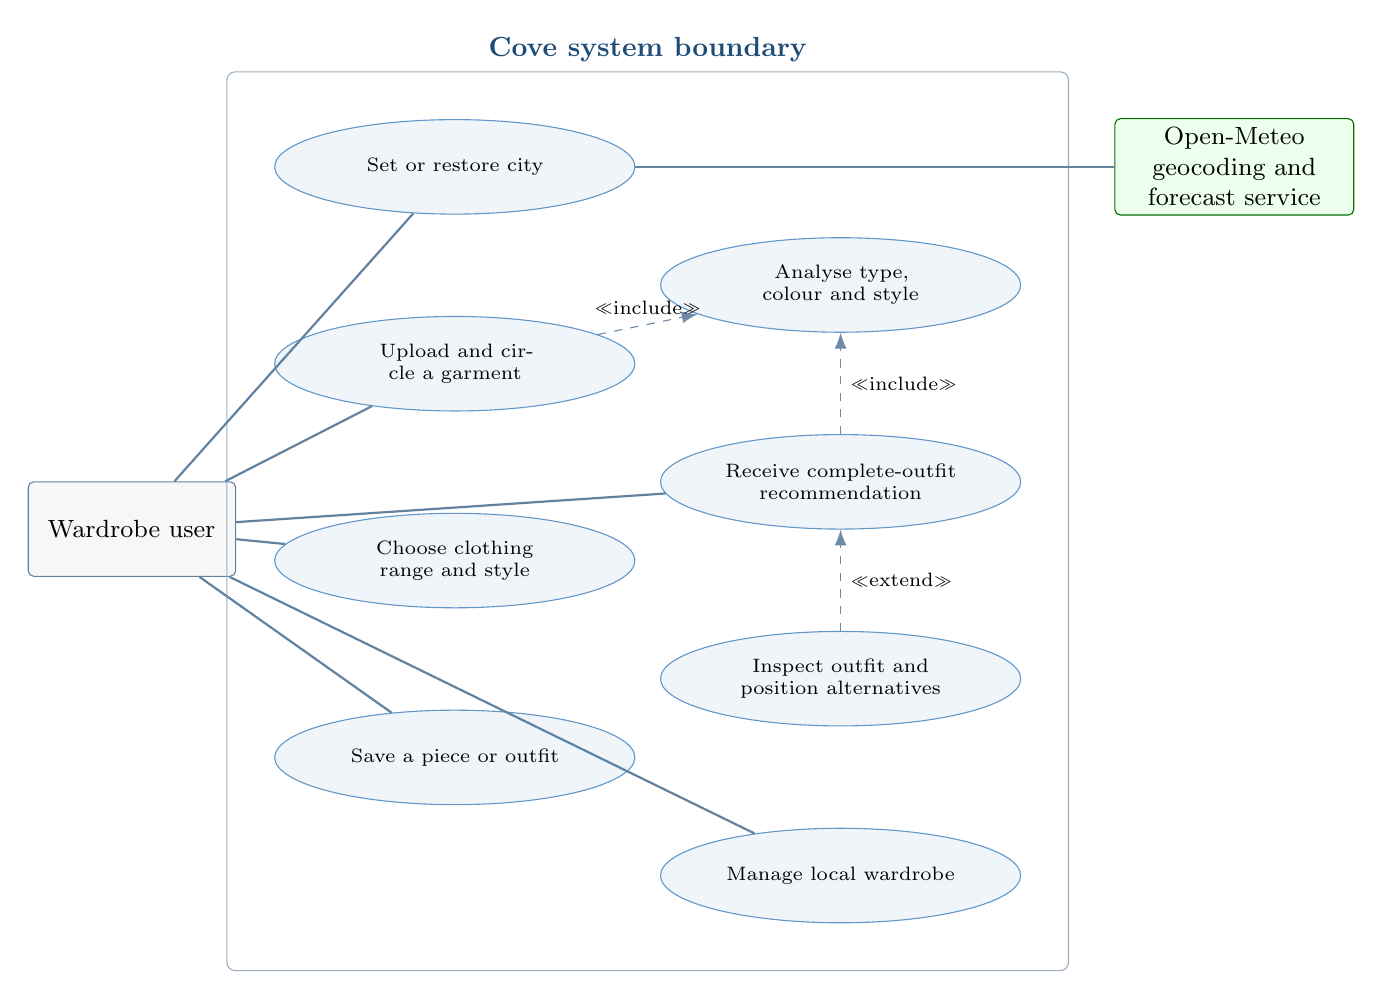
\begin{tikzpicture}[
    font=\small,
    actor/.style={draw=wmgdarkblue!70, rounded corners=2pt, align=center,
      text width=24mm, minimum height=12mm, fill=gray!6},
    usecase/.style={draw=wmgblue!75, ellipse, align=center,
      text width=30mm, minimum height=12mm, fill=wmgblue!7, font=\scriptsize},
    external/.style={draw=green!45!black, rounded corners=2pt, align=center,
      text width=28mm, minimum height=12mm, fill=green!7},
    association/.style={thick, draw=wmgdarkblue!70},
    include/.style={-{Latex[length=2mm]}, dashed, draw=wmgdarkblue!65}
  ]
    \node[actor] (user) at (0,1.0) {Wardrobe user};
    \node[usecase] (city) at (4.1,5.6) {Set or restore city};
    \node[usecase] (select) at (4.1,3.1) {Upload and circle a garment};
    \node[usecase] (analyse) at (9.0,4.1) {Analyse type, colour and style};
    \node[usecase] (context) at (4.1,0.6) {Choose clothing range and style};
    \node[usecase] (recommend) at (9.0,1.6) {Receive complete-outfit recommendation};
    \node[usecase] (save) at (4.1,-1.9) {Save a piece or outfit};
    \node[usecase] (alternatives) at (9.0,-0.9) {Inspect outfit and position alternatives};
    \node[usecase] (manage) at (9.0,-3.4) {Manage local wardrobe};
    \node[external] (weather) at (14.0,5.6) {Open-Meteo geocoding and forecast service};

    \node[draw=wmgdarkblue!45, rounded corners=3pt,
      fit=(city)(select)(analyse)(context)(recommend)(alternatives)(save)(manage),
      inner sep=6mm, label={[font=\bfseries\color{wmgdarkblue}]above:Cove system boundary}] {};

    \draw[association] (user) -- (city);
    \draw[association] (user) -- (select);
    \draw[association] (user) -- (context);
    \draw[association] (user) -- (recommend);
    \draw[association] (user) -- (save);
    \draw[association] (user) -- (manage);
    \draw[association] (weather) -- (city);
    \draw[include] (select) -- node[above,font=\scriptsize]{\guillemotleft include\guillemotright} (analyse);
    \draw[include] (recommend) -- node[right,font=\scriptsize]{\guillemotleft include\guillemotright} (analyse);
    \draw[include] (alternatives) -- node[right,font=\scriptsize]{\guillemotleft extend\guillemotright} (recommend);
  \end{tikzpicture}}
  \caption{UML use-case view of the implemented Cove prototype}
  \label{fig:use-case}
\end{figure}


\section{Overall software structure}

The application is predominantly function-oriented, so an overall class
diagram would invent classes that do not exist. Figure~\ref{fig:overall-architecture}
uses a UML-style component view to show the real source modules, external
service and stored artefacts.

\begin{figure}[htbp]
  \centering
  \resizebox{0.98\textwidth}{!}{%
  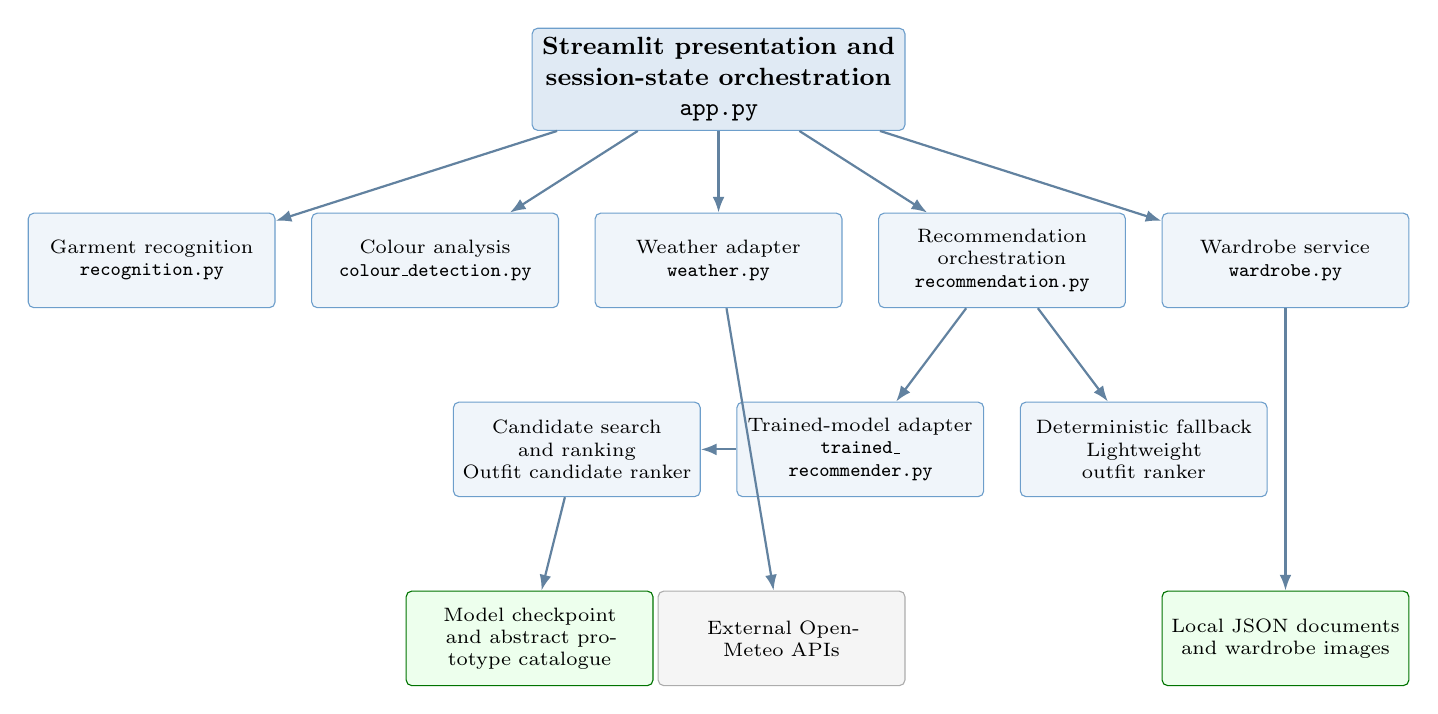
\begin{tikzpicture}[
    font=\small,
    component/.style={draw=wmgblue!70, rounded corners=2pt, align=center,
      text width=29mm, minimum height=12mm, fill=wmgblue!7, font=\scriptsize},
    core/.style={component, fill=wmgblue!15, font=\small\bfseries},
    store/.style={component, fill=green!7, draw=green!45!black},
    external/.style={component, fill=gray!8, draw=gray!65},
    arrow/.style={-{Latex[length=2mm]}, thick, draw=wmgdarkblue!70}
  ]
    \node[core, text width=45mm] (app) at (7.2,6.0) {Streamlit presentation and session-state orchestration\\{\ttfamily app.py}};

    \node[component] (recognition) at (0,3.7) {Garment recognition\\{\ttfamily recognition.py}};
    \node[component] (colour) at (3.6,3.7) {Colour analysis\\{\ttfamily colour\_detection.py}};
    \node[component] (weather) at (7.2,3.7) {Weather adapter\\{\ttfamily weather.py}};
    \node[component] (recommendation) at (10.8,3.7) {Recommendation orchestration\\{\ttfamily recommendation.py}};
    \node[component] (wardrobe) at (14.4,3.7) {Wardrobe service\\{\ttfamily wardrobe.py}};

    \node[component] (trained) at (9.0,1.3) {Trained-model adapter\\{\ttfamily trained\_}\\{\ttfamily recommender.py}};
    \node[component] (fallback) at (12.6,1.3) {Deterministic fallback\\Lightweight outfit ranker};
    \node[component] (ranker) at (5.4,1.3) {Candidate search and ranking\\Outfit candidate ranker};

    \node[store] (modelstore) at (4.8,-1.1) {Model checkpoint and abstract prototype catalogue};
    \node[store] (userstore) at (14.4,-1.1) {Local JSON documents and wardrobe images};
    \node[external] (openmeteo) at (8.0,-1.1) {External Open-Meteo APIs};

    \draw[arrow] (app) -- (recognition);
    \draw[arrow] (app) -- (colour);
    \draw[arrow] (app) -- (weather);
    \draw[arrow] (app) -- (recommendation);
    \draw[arrow] (app) -- (wardrobe);
    \draw[arrow] (recommendation) -- (trained);
    \draw[arrow] (recommendation) -- (fallback);
    \draw[arrow] (trained) -- (ranker);
    \draw[arrow] (ranker) -- (modelstore);
    \draw[arrow] (weather) -- (openmeteo);
    \draw[arrow] (wardrobe) -- (userstore);
  \end{tikzpicture}}
  \caption{Overall UML-style component view of the Cove software}
  \label{fig:overall-architecture}
\end{figure}


\section{Recommendation-module classes and dependencies}

Figure~\ref{fig:recommendation-classes} focuses on the classes that are present
in the recommendation path and includes the function-based adapter and facade
on which they depend.

\begin{figure}[htbp]
  \centering
  \resizebox{0.98\textwidth}{!}{%
  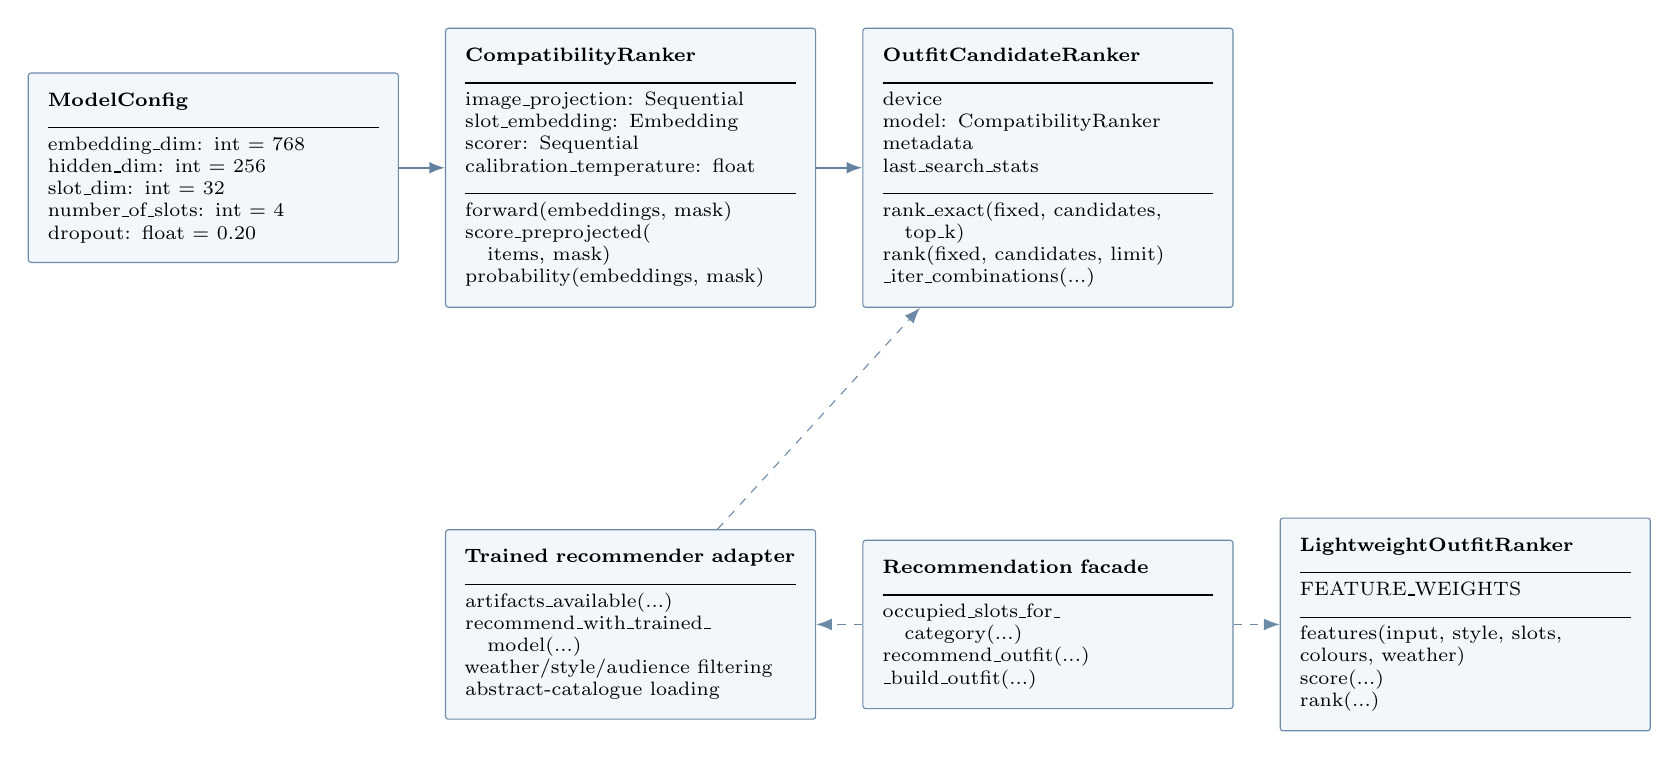
\begin{tikzpicture}[
    font=\scriptsize,
    class/.style={draw=wmgdarkblue!65, rounded corners=1pt, align=left,
      text width=42mm, fill=wmgblue!6, inner sep=2.5mm},
    relation/.style={-{Latex[length=2mm]}, thick, draw=wmgdarkblue!70},
    dependency/.style={-{Latex[length=2mm]}, dashed, draw=wmgdarkblue!65}
  ]
    \node[class] (config) at (0,5.0) {\textbf{ModelConfig}\\\hrulefill\\
      embedding\_dim: int = 768\\hidden\_dim: int = 256\\slot\_dim: int = 32\\number\_of\_slots: int = 4\\dropout: float = 0.20};
    \node[class] (model) at (5.3,5.0) {\textbf{CompatibilityRanker}\\\hrulefill\\
      image\_projection: Sequential\\slot\_embedding: Embedding\\scorer: Sequential\\calibration\_temperature: float\\\hrulefill\\
      forward(embeddings, mask)\\score\_preprojected(\\\quad items, mask)\\probability(embeddings, mask)};
    \node[class] (candidate) at (10.6,5.0) {\textbf{OutfitCandidateRanker}\\\hrulefill\\
      device\\model: CompatibilityRanker\\metadata\\last\_search\_stats\\\hrulefill\\
      rank\_exact(fixed, candidates,\\\quad top\_k)\\rank(fixed, candidates, limit)\\\_iter\_combinations(...)};

    \node[class] (adapter) at (5.3,-0.8) {\textbf{Trained recommender adapter}\\\hrulefill\\
      artifacts\_available(...)\\recommend\_with\_trained\_\\\quad model(...)\\weather/style/audience filtering\\abstract-catalogue loading};
    \node[class] (facade) at (10.6,-0.8) {\textbf{Recommendation facade}\\\hrulefill\\
      occupied\_slots\_for\_\\\quad category(...)\\recommend\_outfit(...)\\\_build\_outfit(...)};
    \node[class] (fallback) at (15.9,-0.8) {\textbf{LightweightOutfitRanker}\\\hrulefill\\
      FEATURE\_WEIGHTS\\\hrulefill\\
      features(input, style, slots, colours, weather)\\score(...)\\rank(...)};

    \draw[relation] (config) -- (model);
    \draw[relation] (model) -- (candidate);
    \draw[dependency] (adapter) -- (candidate);
    \draw[dependency] (facade) -- (adapter);
    \draw[dependency] (facade) -- (fallback);
  \end{tikzpicture}}
  \caption{Module-level UML class and dependency diagram for recommendation}
  \label{fig:recommendation-classes}
\end{figure}


\section{Logical entity relationships}

Figure~\ref{fig:persistence-erd} expresses the multiplicities in the local
wardrobe schema. It is an entity-relationship view of serialised application
state, not evidence of a relational database implementation.

\begin{figure}[htbp]
  \centering
  \resizebox{0.96\textwidth}{!}{%
  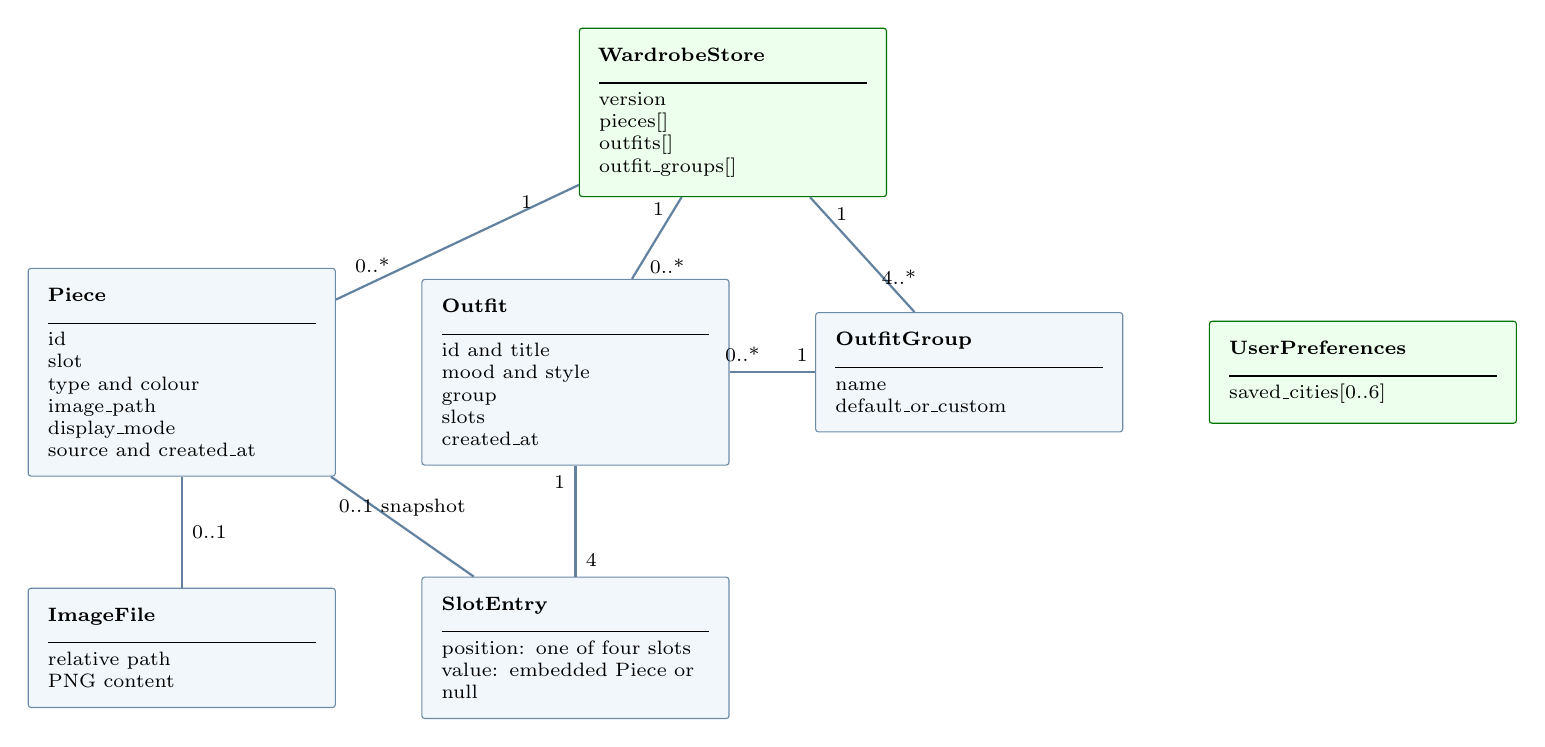
\begin{tikzpicture}[
    font=\scriptsize,
    entity/.style={draw=wmgdarkblue!65, rounded corners=1pt, align=left,
      text width=34mm, fill=wmgblue!6, inner sep=2.5mm},
    store/.style={entity, fill=green!7, draw=green!45!black},
    rel/.style={thick, draw=wmgdarkblue!70}
  ]
    \node[store] (wardrobe) at (7.0,6.0) {\textbf{WardrobeStore}\\\hrulefill\\version\\pieces[]\\outfits[]\\outfit\_groups[]};
    \node[entity] (piece) at (0,2.7) {\textbf{Piece}\\\hrulefill\\id\\slot\\type and colour\\image\_path\\display\_mode\\source and created\_at};
    \node[entity] (outfit) at (5.0,2.7) {\textbf{Outfit}\\\hrulefill\\id and title\\mood and style\\group\\slots\\created\_at};
    \node[entity] (group) at (10.0,2.7) {\textbf{OutfitGroup}\\\hrulefill\\name\\default\_or\_custom};
    \node[store] (preferences) at (15.0,2.7) {\textbf{UserPreferences}\\\hrulefill\\saved\_cities[0..6]};
    \node[entity] (image) at (0,-0.8) {\textbf{ImageFile}\\\hrulefill\\relative path\\PNG content};
    \node[entity] (slot) at (5.0,-0.8) {\textbf{SlotEntry}\\\hrulefill\\position: one of four slots\\value: embedded Piece or null};

    \draw[rel] (wardrobe) -- node[pos=0.15,left,font=\scriptsize]{1} node[pos=0.85,above,font=\scriptsize]{0..*} (piece);
    \draw[rel] (wardrobe) -- node[pos=0.15,left,font=\scriptsize]{1} node[pos=0.85,right,font=\scriptsize]{0..*} (outfit);
    \draw[rel] (wardrobe) -- node[pos=0.15,right,font=\scriptsize]{1} node[pos=0.85,above,font=\scriptsize]{4..*} (group);
    \draw[rel] (outfit) -- node[pos=0.15,left,font=\scriptsize]{1} node[pos=0.85,right,font=\scriptsize]{4} (slot);
    \draw[rel] (slot) -- node[above,font=\scriptsize]{0..1 snapshot} (piece);
    \draw[rel] (piece) -- node[right,font=\scriptsize]{0..1} (image);
    \draw[rel] (group) -- node[pos=0.15,above,font=\scriptsize]{1} node[pos=0.85,above,font=\scriptsize]{0..*} (outfit);
  \end{tikzpicture}}
  \caption{Entity-relationship view of the logical file schema; these entities are serialised to JSON rather than relational tables}
  \label{fig:persistence-erd}
\end{figure}


\section{User stories and acceptance criteria}

Table~\ref{tab:user-stories} converts the implemented interaction paths into
testable user stories. Priorities distinguish the core recommendation journey
from supporting convenience features.

\begingroup
\scriptsize
\setlength{\tabcolsep}{3pt}
\renewcommand{\arraystretch}{1.18}
\begin{longtable}{@{}p{0.06\textwidth}p{0.13\textwidth}p{0.29\textwidth}p{0.38\textwidth}p{0.07\textwidth}@{}}
  \caption{Implemented user stories and acceptance criteria}\label{tab:user-stories}\\
  \toprule
  \textbf{ID} & \textbf{Feature} & \textbf{User story} & \textbf{Acceptance criteria} & \textbf{Priority} \\
  \midrule
  \endfirsthead
  \multicolumn{5}{l}{\textit{Table~\thetable\ continued}}\\
  \toprule
  \textbf{ID} & \textbf{Feature} & \textbf{User story} & \textbf{Acceptance criteria} & \textbf{Priority} \\
  \midrule
  \endhead
  \bottomrule
  \endfoot
  US-01 & Location & As a user, city weather should inform the outfit context. & A valid city returns current conditions; an invalid or unavailable request produces a bounded error rather than stopping the application. & Must \\
  US-02 & Saved cities & As a user, frequently used cities should be available without retyping. & A city can be saved or removed; no more than six are retained; selecting one refreshes the forecast. & Should \\
  US-03 & Image selection & As a user, a garment should be selectable from a photograph. & The user can upload an image, draw a region and repeat the selection before analysis. & Must \\
  US-04 & Recognition & As a user, the selected garment should be interpreted before recommendation. & The application returns a supported broad category, colour, style cues and an image embedding, with an editable fallback when recognition is uncertain. & Must \\
  US-05 & Context control & As a user, clothing range and style should remain under explicit control. & Menswear or womenswear and an available style can be selected; changing either regenerates the recommendation without inferring gender from the image. & Must \\
  US-06 & Outfit completion & As a user, the selected garment should remain fixed while the outfit is completed. & The result covers all feasible supported positions, respects occupied slots and weather constraints, and uses product-independent types and colours. & Must \\
  US-07 & Alternatives & As a user, more than one acceptable solution should be inspectable. & The interface provides a primary outfit, a materially different alternative and model-ranked position replacements where feasible. & Must \\
  US-08 & Operational fallback & As a user, recommendation should remain available if model artefacts cannot load. & The system records the loading reason and returns a deterministic rule-ranked result without presenting it as a learned score. & Must \\
  US-09 & Save result & As a user, either the supplied garment or a complete recommendation should be saved. & Saving preserves the user image where available and represents abstract recommended garments as coloured icons. & Should \\
  US-10 & Outfit editing & As a user, saved outfits should be completed and revised later. & Each of four equal positions supports add, replace or confirmed removal; an outfit can be renamed and assigned to a group. & Should \\
  US-11 & Piece library & As a user, individual garments should be reusable across outfits. & Pieces can be filtered by four positions, renamed, reused in multiple outfits and deleted with confirmation. & Should \\
  US-12 & Local persistence & As a user, wardrobe information should remain private on the device. & Wardrobe JSON, preferences and images are stored locally and are not incorporated into model training. & Must \\
\end{longtable}
\endgroup


\end{document}
